\documentclass{article}

% PACKAGES
% General Formatting & Language
\usepackage[english]{babel}
\usepackage[letterpaper,top=2cm,bottom=2cm,left=3cm,right=3cm,marginparwidth=1.75cm]{geometry}
\usepackage{booktabs}
\usepackage{longtable}
\usepackage{multirow}
\usepackage{float}
\usepackage{placeins}


% Math & Symbols
\usepackage{amsmath}
\usepackage{amssymb}
\usepackage{amsthm}
\usepackage{bm}
\usepackage{bbold}

% Graphics & Colors
\usepackage{graphicx}
\usepackage{xcolor}
\usepackage[most]{tcolorbox}

% TikZ
\usepackage{tikz}
\usetikzlibrary{shapes, decorations.pathmorphing, shapes.geometric, calc, arrows.meta, positioning, backgrounds}
\usetikzlibrary{matrix,positioning,calc}


% Algorithms
\usepackage{algorithm}
\usepackage{algorithmic}

% Miscellaneous
\usepackage{enumitem}
\usepackage{url}
\usepackage[colorlinks=true, allcolors=blue]{hyperref}

% CUSTOM COMMANDS & THEOREMS
\newtheorem{lemma}{Lemma}
\newcommand{\hlm}[1]{{\color{blue}#1}}
\newcommand{\mbw}[1]{{\color{blue}#1}}
\newcommand{\ind}{\mathrel{\perp\!\!\!\!\perp}}

\title{CICADAS: A Simulation-Based Framework for Randomized Trial Emulation in Critical-Care Seizure Treatment}


% \title{CICADAS \cicada: A Simulation-Based Tutorial for Causal Survival Analysis with Complex Time-Varying Confounding}

% \title{CICADAS: A Simulation-Based Tutorial for Causal Survival Analysis with Complex Time-Varying Confounding}


\author{
    Mitchell McCauley\textsuperscript{1*},
    Tara Westover\textsuperscript{2*}, 
    Patrick Wynn\textsuperscript{1*}, 
    Shadi Sartipi\textsuperscript{3*}, \\
    Niels Turley\textsuperscript{1},
    Zade Akras\textsuperscript{3},
    Pieter Colin\textsuperscript{4},
    Andrew Webb\textsuperscript{3}, 
    Aaron F. Struck\textsuperscript{5},
    Jennifer Kim\textsuperscript{6},\\ 
    David Cheng\textsuperscript{3}, % Manual line break for formatting
    Haoqi Sun\textsuperscript{1}, 
    Tim Houle\textsuperscript{3}, 
    Cynthia Rudin\textsuperscript{7}, 
    Alexander Volfovsky\textsuperscript{7}, Harsh Parikh\textsuperscript{6} \\
    Marta B. Fernandes\textsuperscript{3\dag}, % Manual line break for formatting
    Sahar Zafar\textsuperscript{3\dag},
    M.\ Brandon Westover\textsuperscript{1\dag}
}

\date{} % Suppress date

\begin{document}

\maketitle

% Author contributions and affiliations
% Note: The \footnotetext commands provide the text for the symbols (*, †) in the author list.
\begingroup
\renewcommand\thefootnote{\fnsymbol{footnote}}
\footnotetext[1]{Co-first authors.}
\footnotetext[2]{Co-senior authors.}
\endgroup

% Affiliation list
\begingroup
\small
\noindent\textsuperscript{1}Beth Israel Deaconess Medical Center / Harvard Medical School\\
\textsuperscript{2}Harvard University\\
\textsuperscript{3}Massachusetts General Hospital / Harvard Medical School\\
\textsuperscript{4}Rijksuniversiteit Groningen\\
\textsuperscript{5}Washington University School of Medicine\\
\textsuperscript{6}Yale University\\
\textsuperscript{7}Duke University

\par
\endgroup

\begin{abstract}
Non-convulsive seizures affect approximately 30\% of critically ill patients who undergo EEG
monitoring, yet optimal treatment strategies remain uncertain because of the trade-off between
seizure suppression and drug toxicity. Randomized trials in this setting are expensive, ethically
fraught, and have so far been inconclusive, while the wide practice variation in routine ICU care
creates observational data in which treatment decisions and disease progression influence each other
over time---a confounding structure that defeats standard survival analysis.

We present CICADAS (\textbf{C}ausal \textbf{I}nference for \textbf{C}ritical-Care
\textbf{A}nti-Seizure Treatment with \textbf{D}isease Dynamics, \textbf{A}utomated PKPD/Trial
Simulation, and \textbf{S}urvival Optimization), a computational framework that couples the
parametric g-formula with mechanistic pharmacokinetic--pharmacodynamic modeling, disease dynamics,
and dynamic treatment policies to emulate randomized trials from longitudinal observational data. We
specify the notation and identification assumptions required for time-varying treatment and
confounding, describe a sequential estimation procedure for each model component, and provide open
implementations in MATLAB and Python.

The framework is evaluated entirely by \emph{internal, simulation-based validation} on synthetic ICU
cohorts with known ground truth. Across 400 simulated replications, confounding by indication
attenuated a true 14.6 percentage-point survival benefit to 1.0 points under naive Kaplan--Meier
analysis---eliminating 93\% of the effect---and reversed its sign in 39\% of replications. Under
these conditions the g-formula recovers the ground-truth treatment effect closely, whereas naive
Kaplan--Meier, stabilized inverse probability of treatment weighting, and a baseline-weighted
marginal structural model do not. We report the estimator's
behavior under injected unmeasured confounding, EEG measurement error, and alternative censoring
mechanisms.

These results establish methodological feasibility, not clinical utility. Because the simulated data
and the estimation models share structural assumptions, the recovery results characterize estimator
consistency under correct specification rather than robustness to misspecification. Whether CICADAS
yields valid causal estimates in real ICU data is an open question, to be addressed by external
validation in multicenter ICU EEG cohorts.
\end{abstract}

\section{Introduction}

Non-convulsive seizures occur in about 30\% of critically ill patients who undergo electroencephalography (EEG) monitoring~\cite{hirsch2021american} and are associated with  prolonged intensive care unit (ICU) stays, high healthcare costs, increased mortality, and long-term neurological impairment~\cite{rodriguez2017association,vespa2005continuous,westover2015probability}. Despite increased detection owing to widespread use of continuous EEG monitoring, optimal treatment strategies remain uncertain: Aggressive anti-seizure therapy can suppress epileptiform activity, but carries risks of sedation, hemodynamic instability, and drug toxicity, while untreated seizures may damage the brain~\cite{lalgudi2019electrographic, demarchis2016seizure, payne2014seizure, zafar2018effect, rossetti2005refractory, muhlhofer2019duration, marchi2015status, an2018variability, sutter2016status, abend2015critical}. 

This uncertainty leads to practice variation across clinicians and institutions, illustrated in Figure~\ref{fig:control-problem}. Some centers and some clinicians routinely use aggressive anti-seizure therapy, while others adopt more conservative approaches~\cite{chong2005which, rubinos2018ictal, osman2018ictal, johnson2017population, tao2020ictal, cormier2017ictal}. This variability, while reflecting uncertainty about optimal care, nevertheless provides an opportunity to learn, from observational data, which treatment strategies lead to the best outcomes. However, extracting valid causal insights from this variation is far from straightforward. Treatment decisions and disease progression influence each other over time in a feedback loop, creating two particularly acute statistical challenges. First, confounding by indication, where sicker patients are more likely to receive aggressive treatment, making treatment appear harmful when it may in fact be beneficial. Second, time-varying confounding with treatment–confounder feedback, where treatment at one time point affects subsequent disease severity, which in turn influences later treatment decisions and treatment response (e.g., electrographic improvement or adverse effects).

Experimental studies such as randomized controlled trials (RCTs) could provide valid treatment effect estimation. However, operationalizing them in critical-care seizure management is challenging due to ethical, financial, and logistical constraints. When there is substantial uncertainty about the risks related to a given treatment strategy, an RCT risks enrolling large numbers of patients into a protocol that may be ineffective or even harmful.

The two RCTs that have studied aggressive anti-seizure treatment in critically ill adults---Husain et al.~\cite{husain2018randomized} in non-convulsive status epilepticus and Ruijter et al.~\cite{ruijter2022treating} in rhythmic or periodic EEG patterns following post-anoxic encephalopathy---both reported null results for the primary outcomes. We do not claim that these null results can be explained away by a single cause. They may reflect a genuine absence of a population-average effect in the populations studied, features of the specific dosing protocols and trial designs, heterogeneity of the underlying disease, or some combination. The post-anoxic encephalopathy population in particular has a pathophysiology in which widespread ischemic injury may render any seizure-directed therapy futile regardless of protocol.

What CICADAS can contribute is orthogonal to re-litigating those null results: given the uncertainty about when and in whom EA-directed treatment is beneficial, we use causal inference on observational data---where treatment intensity varies substantially across patients, clinicians, and centers---to identify the patient subgroups and treatment intensities in which a benefit is most plausible. These subgroup-specific hypotheses are intended as inputs to the design of focused future trials rather than as contradictions of existing ones~\cite{parikh2024many}.

Because randomized controlled trials are difficult to conduct and may not capture the complexity of ICU seizure management, an alternative approach is to learn from the wealth of observational data collected in routine ICU care. However, drawing valid causal conclusions from such data is methodologically challenging. Standard regression or Kaplan–Meier analyses can be biased when treatment and disease severity influence each other over time. Modern causal inference methods—particularly the parametric g-formula—offer a principled way to overcome these challenges by modeling the joint distribution of time-varying variables and simulating counterfactual outcomes under hypothetical treatment strategies~\cite{hernan2016using, hernan2020causal, parikh2024many}.

Our work builds on two prior studies of seizure treatment in the ICU~\cite{parikh2023effects, parikh2024safe}. The first~\cite{parikh2023effects} used PK/PD modeling and matching in retrospective ICU EEG data to estimate a causal harmful effect of epileptiform activity (EA) on outcomes after accounting for EA--treatment feedback. That evidence is consistent with, but does not definitively establish, a causal role for EA: it rests on a single retrospective cohort and remains subject to residual unmeasured confounding, and the generalizability of the effect across patient subgroups and seizure etiologies is not yet known. Treating EA reduction as a provisional therapeutic target---rather than an established one---is one of the motivations for the simulation-based hypothesis-generating framework presented here. The second study~\cite{parikh2024safe} examined whether outcomes could be improved by selecting, for a given patient, among treatment patterns already observed in routine practice those associated with the highest probability of favorable outcomes. That work fit a simplified policy template to observed clinical care and introduced useful new methodology; a key limitation was that the fitted policies only modestly captured actual clinician behavior. The present work (CICADAS) advances this trajectory by moving beyond simplified policy templates to closed-loop seizure treatment strategies that more closely reflect physiologic dynamics. By integrating the parametric g-formula with mechanistic PK/PD models, disease dynamics, and simulated randomized trials, CICADAS is designed to generate physiologically plausible dynamic control targets as hypotheses for prospective evaluation rather than as direct clinical recommendations.

Here we build on this literature to present a computational framework for \emph{posing} the question of optimal seizure management as a formal causal estimation problem, and we evaluate, in simulation, whether that problem can be solved when the data-generating process is known. Our paper makes four contributions:
\begin{enumerate}
\item \textbf{Clinical motivation}: We formalize the question of optimal anti-seizure treatment in the ICU as a dynamic-treatment-regime problem, in a setting where randomized trials are impractical and the two that have been conducted were inconclusive. The framework is intended to generate hypotheses for such trials, not to guide individual treatment decisions.

\item \textbf{Methodological bridge}: We present a comprehensive tutorial with detailed mathematical derivations that connect modern causal inference theory to the practical challenges of estimating treatment effects in ICU seizure management, where treatment decisions and disease dynamics interact over time.

\item \textbf{Simulation framework with known ground truth}: We develop CICADAS (Causal Inference for Critical Care with Adherence, Disease dynamics, and Survival), a realistic simulation platform that captures seizure disease dynamics and pharmacokinetic--pharmacodynamic effects of anti-seizure medications. All analyses in this paper are performed on simulated data in which the true causal effects are known, enabling rigorous validation of the methods under controlled conditions.

\item \textbf{Exploration of the policy space}: Using the simulated cohorts, we illustrate how the framework can be used to compare a family of closed-loop policies indexed by the target threshold $\theta$, and how the comparison varies with simulated patient characteristics. These are demonstrations of what the machinery computes, within a data-generating process we specified; they are not findings about patients. External validation in real ICU EEG cohorts is required before any such comparison carries clinical meaning, and is the subject of separate, ongoing work.
\end{enumerate}

By bridging causal inference theory with clinically realistic modeling, CICADAS is intended as a framework for \textbf{targeted hypothesis generation} from observational ICU datasets. Rather than replacing randomized trials, the approach is designed to help allocate trial resources by identifying the patient subgroups and treatment intensities in which a benefit is most plausible. Whether it can do so in real data is the subject of Section~\ref{sec:external-validation} and remains untested.

The paper proceeds as follows. Section~\ref{sec:clinical-problem} states the clinical control problem
and fixes notation; Sections~\ref{sec:prelim}--\ref{sec:estimation} develop the causal framework, the
simulation model, and the estimation procedure; Section~\ref{sec:results} reports the simulation study,
including internal validation, methodological benchmarking, and robustness analyses; and
Sections~\ref{sec:discussion}--\ref{sec:conclusion} discuss what the framework can and cannot support.
Derivations, full model parameterizations, and estimation details are given in the Supplementary Material.

\section{The Clinical Control Problem}
\label{sec:clinical-problem}

Identifying an optimal seizure-management strategy requires more than describing which patients do
well. It requires representing seizure treatment as what it is in practice: a dynamic control
problem, in which clinicians repeatedly observe electrographic disease burden and adjust
anti-seizure medication in response, so that treatment and disease evolution shape one another over
time. This section states the problem and fixes the notation used for the rest of the paper. It
deliberately stops short of any result; the framework is developed in Sections~\ref{sec:prelim}--\ref{sec:estimation}
and evaluated in Section~\ref{sec:results}.

\subsection{Notation}
\label{sec:notation}

We observe patients at discrete times $t \in \{0,1,2,\ldots\}$ over a 168-hour horizon, and write
$\bar{Z}_t$ for the history of a variable $Z$ through time $t$.

\begin{itemize}\setlength{\itemsep}{2pt}
\item $L_t$ --- \textbf{epileptiform-activity burden}, a scalar summary of EEG severity at time $t$.
This is the quantity clinicians titrate against, and the input to the feedback controller defined
below. Section~\ref{sec:eeg-readout} discusses what is lost in reducing an EEG to a scalar, and what
a real deployment would require of this measurement.

\item $L_{0,t}$ --- the \textbf{natural history}: the burden that would have been observed at time
$t$ under no treatment. $L_t$ and $L_{0,t}$ coincide in untreated patients and diverge under
therapy.

\item $X$ --- baseline clinical covariates (age, SOFA score).

\item $A_t$ --- treatment intensity at time $t$; a continuous, non-negative infusion rate.

\item $\theta$ --- the \textbf{target epileptiform-activity threshold}: the level of $L_t$ that a
given treatment policy attempts to maintain. A policy is indexed by $\theta$; smaller $\theta$ means
more aggressive suppression.

\item $C_{t+1}$, $Y_{t+1}$ --- censoring and death indicators for the interval $(t,t+1]$.

\item $H_t = (X, \bar{L}_t, \bar{A}_{t-1})$ --- the \textbf{observed history} through time $t$:
baseline covariates together with all severity measurements and all treatment decisions made up to
that point. This is the conditioning set on which the identification assumptions of
Section~\ref{sec:prelim} are stated.
\end{itemize}

The distinction between $L_t$ and $H_t$ is used throughout and is worth stating once explicitly. A
treatment policy is a rule for setting $A_t$ from the current scalar severity $L_t$---that is what a
clinician titrating at the bedside actually does. Valid causal identification, by contrast, requires
conditioning on the entire history $H_t$, including baseline covariates and past treatment. The two
objects serve different purposes: $L_t$ defines \emph{what the policy is}, and $H_t$ defines
\emph{what must be adjusted for} in order to estimate the policy's effect.

\subsection{Variation in Clinical Practice}

Figure~\ref{fig:control-problem}A--C shows three treatment patterns commonly seen in ICU care. The
untreated patient (panel A) follows the natural history---a characteristic rise and fall that,
though eventually self-resolving, often proves fatal before resolution; this occurs when the
treating physician judges treatment more harmful than beneficial. The dose-changing patient (panel
B) receives intermittent adjustments. The closed-loop patient (panel C) is titrated continuously to
hold burden below a target ($\theta = 0.1$ in this illustration).

The intermittent adjustments in panel B are not meant to suggest arbitrary decision-making. They
reflect the episodic, coarse changes that arise from sedation interruptions for neurologic
examination, delayed response to evolving EEG findings, clinician hand-offs, and the absence of
automated titration. Collectively these patterns reflect the absence of consensus on treatment
strategy~\cite{chong2005which, rubinos2018ictal, osman2018ictal, johnson2017population, tao2020ictal, cormier2017ictal}---and
it is precisely this variation that makes observational learning possible, since a population in
which every patient were treated identically would carry no information about alternatives.

\subsection{Closed-Loop Feedback Control}

We take closed-loop control as the natural class of treatment strategies to study. Such a policy
adjusts medication to give no more and no less than needed to keep epileptiform activity below a
target level~\cite{astrom2010feedback, an2017design, westover2015robust, fialho2009closed};
Figure~\ref{fig:control-problem}D gives the schematic. The clinical team is modeled as a controller
that sets treatment intensity $A_t$ from the error $e_t = L_t - \theta$ between observed burden and
target. The patient's response is governed by their natural history $L_{0,t}$ and their individual
pharmacokinetic--pharmacodynamic (PKPD) profile. The result is a closed loop in which treatment and
disease activity are each a function of the other's history.

Two consequences follow, and they organize the rest of the paper. First, within this class,
\emph{asking what treatment is optimal reduces to asking what value of $\theta$ is optimal}---the
search over strategies becomes a search over a single interpretable parameter. Second, the same
feedback that makes the policy clinically sensible is what makes the data hard to analyze: because
$A_t$ depends on $L_t$, and $L_t$ depends on $\bar{A}_{t-1}$, disease severity is simultaneously a
confounder of later treatment and a mediator of earlier treatment. Conditioning on it introduces
bias; ignoring it introduces bias. This is the structure that the g-formula, introduced in
Section~\ref{sec:prelim}, is designed to handle, and that standard adjustment cannot.

\begin{figure}[htbp]
\centering
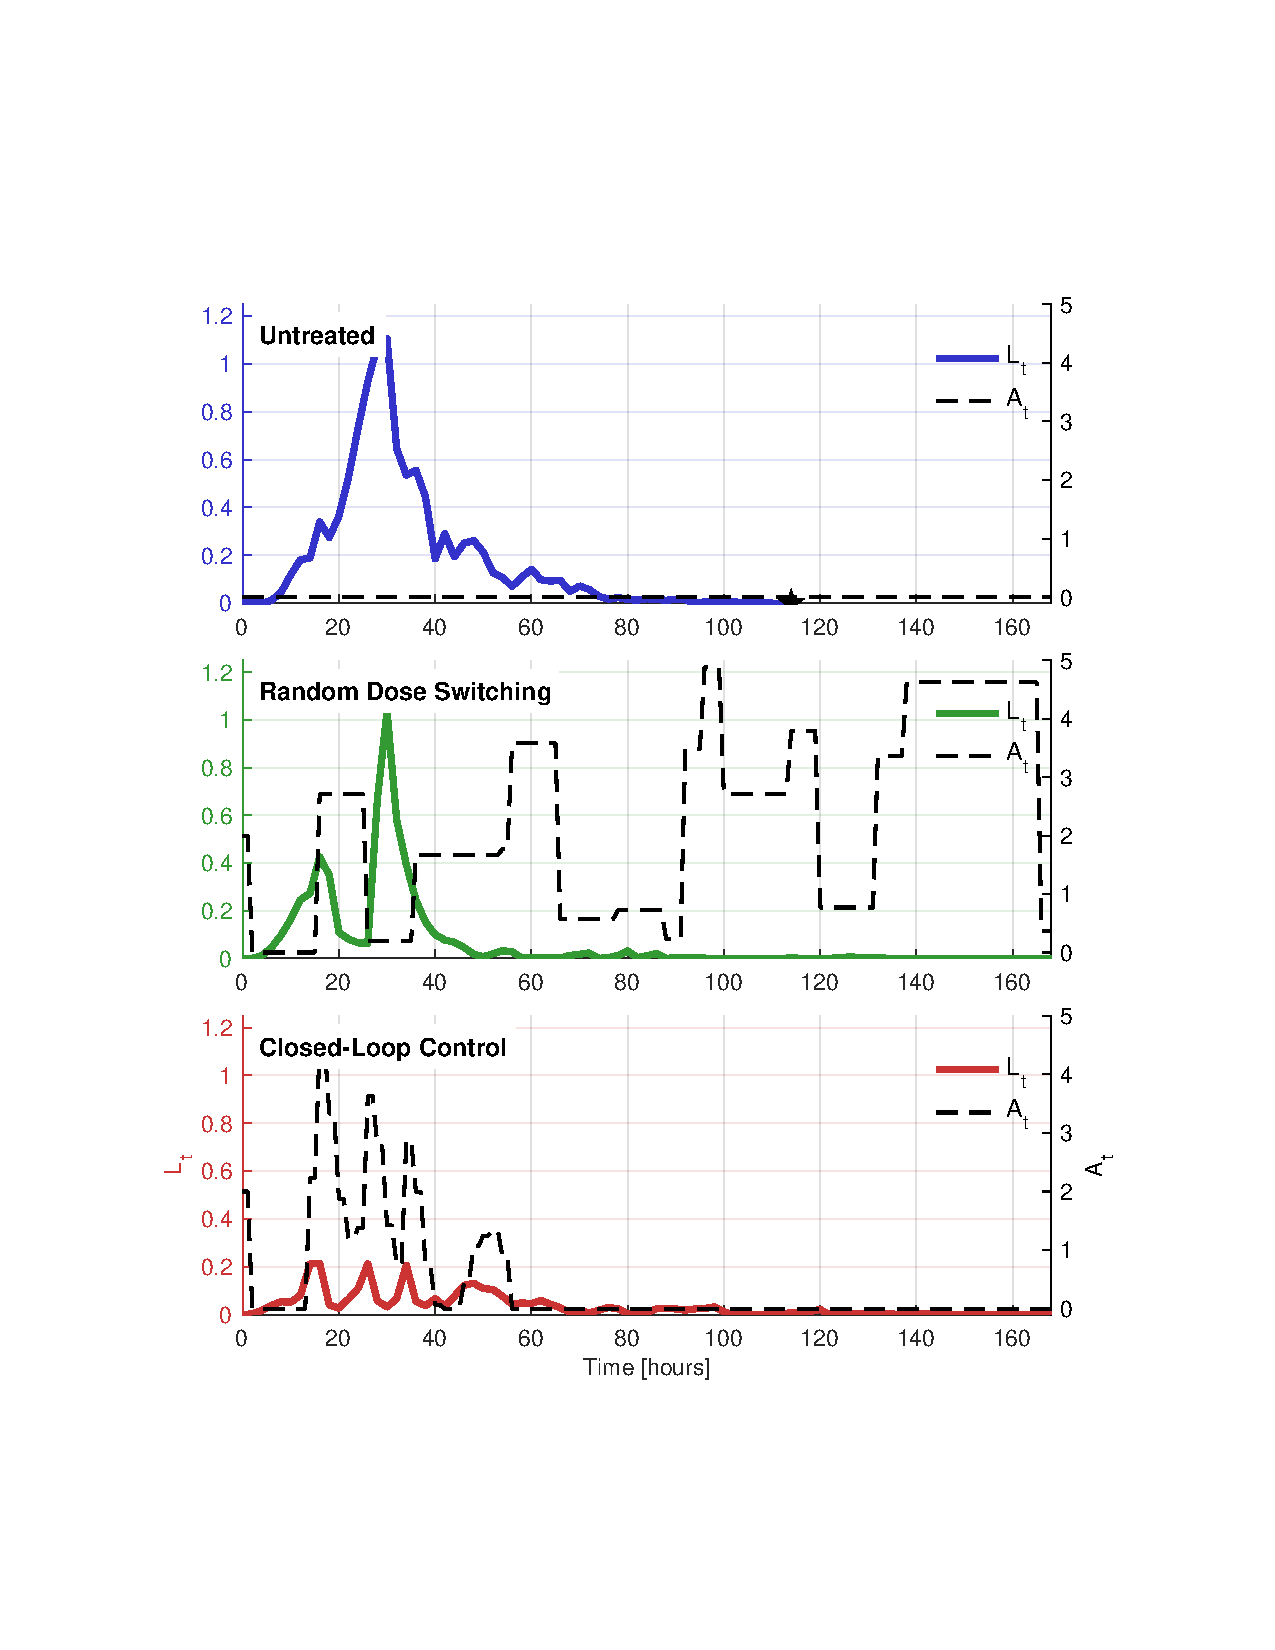
\includegraphics[width=\linewidth, trim=2.25cm 4.5cm 2.25cm 2cm, clip]{Fig1_singleTrajectories_3panels.pdf}

\vspace{1.5em}

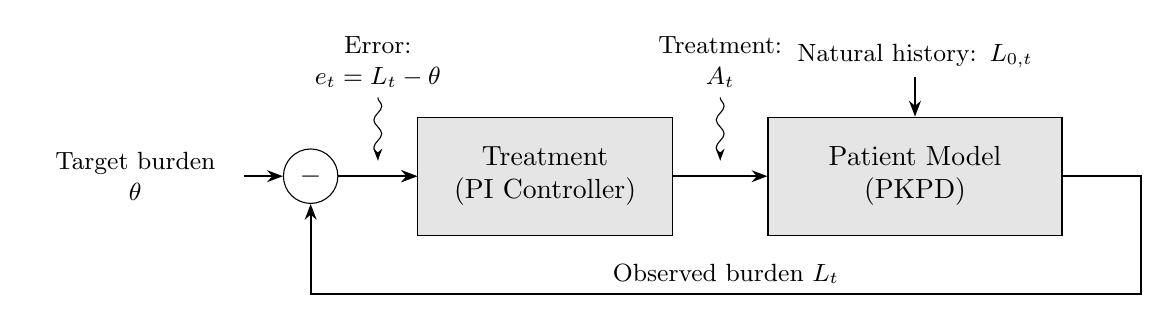
\begin{tikzpicture}[
  block/.style={rectangle, draw, fill=gray!20, text width=3.5cm, text centered, minimum height=1.5cm},
  smallblock/.style={rectangle, draw, fill=gray!20, text width=3cm, text centered, minimum height=1.5cm},
  sum/.style={circle, draw, minimum size=0.5cm},
  arrow/.style={-{Stealth[length=2mm]}, thick},
  label/.style={text width=2.5cm, align=center, font=\small}
]
\node[label] (target) {Target burden\\$\theta$};
\node[sum, right=0.5cm of target] (sumnode) {$-$};
\node[smallblock, right=1cm of sumnode] (controller) {Treatment\\(PI Controller)};
\node[block, right=1.2cm of controller] (patient) {Patient Model\\(PKPD)};
\node[label, text width = 4.7cm, above=0.5cm of patient] (disease)
{Natural history: $L_{0,t}$};
\draw[arrow] (target) -- (sumnode);
\draw[arrow] (sumnode) -- (controller);
\draw[arrow] (controller) -- node[above=10mm, font=\small, align=center] (treatment) {Treatment:\\ $A_t$} (patient);
\draw[arrow] (disease.south) -- (patient.north);
\draw[arrow] (patient.east) -- ++(1,0) |- ++(0,-1.5) -| node[above, font=\small, pos=0.25] {Observed burden $L_t$} (sumnode);
\draw[arrow] (sumnode) -- node[above=10mm, font=\small, align=center] (error) {Error:\\$e_t = L_t - \theta$} (controller);
\draw[decorate, decoration={snake, amplitude=0.5mm}, -{Stealth[length=1.5mm]}, thin]
  (error.south) -- ([yshift=-8mm]error.south);
\draw[decorate, decoration={snake, amplitude=0.5mm}, -{Stealth[length=1.5mm]}, thin]
  (treatment.south) -- ([yshift=-8mm]treatment.south);
\end{tikzpicture}

\caption{\textbf{The seizure-treatment control problem.} \textbf{(A--C)} Epileptiform-activity
burden and treatment intensity over a 168-hour follow-up for three exemplar simulated patients,
illustrating treatment patterns commonly seen in ICU practice. (A) An untreated patient: burden
$L_t$ (solid blue) with $A_t = 0$ (dashed black); the black star marks death ($Y_t = 1$). (B) A
dose-changing patient: $L_t$ (solid green) with time-varying $A_t$ (dashed black), illustrating
intermittent dosing. (C) A patient under closed-loop control: $L_t$ (solid red) with $A_t$ (dashed
black), showing frequent adjustment of treatment intensity to hold burden below a target
epileptiform-activity threshold of $\theta = 0.1$. Left and right vertical axes are scaled for
burden and treatment intensity respectively; the horizontal axis is time in hours. \textbf{(D)}
Feedback representation of the same system. The clinical team, modeled as a proportional--integral
controller, sets treatment $A_t$ from the error $e_t = L_t - \theta$ between observed burden and the
target threshold; the patient's response depends on the untreated natural history $L_{0,t}$ and on
individual PKPD parameters. All trajectories are simulated.}
\label{fig:control-problem}
\end{figure}

\FloatBarrier

\section{Preliminaries}
\label{sec:prelim}

\subsection{Causal Effect of Anti-Seizure Medication}

Here we formalize the problem of estimating causal effects from observational longitudinal
data with time-varying confounding and treatment--confounder feedback loops
\cite{parikh2023effects,hernan2020causal,young2020causal,young2011comparative,wanis2024grace,robins2009estimation}.
We consider a longitudinal study observed at discrete times $t \in \{0,1,2,\ldots\}$.
Throughout, we use bar notation $\bar X_t$ to denote the history of a variable $X$ up to
time $t$.

\paragraph{Observed data.}
The variables involved in the analysis are:
\begin{itemize}
\item $L_t$: The scalar burden of epileptiform activity (EA) measured from EEG at time
$t$, as defined in Section~\ref{sec:notation}. This is the quantity the treatment policy
titrates against. We write $\bar L_t = (L_0,L_1,\ldots,L_t)$. For concreteness, $L_t$
may be operationalized as the seizure burden per monitoring epoch.

\item $X$: Static baseline clinical characteristics (e.g., age, SOFA score).

\item $H_t = (X,\bar L_t,\bar A_{t-1})$: The observed history through time $t$. This is
the conditioning set used in the identification assumptions below. Note the distinction
maintained throughout: policies are functions of the scalar $L_t$, whereas identification
conditions on the full history $H_t$.

\item $A_t$: Treatment administered at time $t$. In our clinical setting, this is a
continuous, nonnegative infusion rate (e.g., propofol infusion). We write
$\bar A_t = (A_0,A_1,\ldots,A_t)$.

\item $C_{t+1}$: Indicator of censoring during the interval $(t,t+1]$, where
$C_{t+1}=1$ if censoring occurs in $(t,t+1]$ and $C_{t+1}=0$ otherwise. Thus,
$\bar C_t=(C_1,\ldots,C_t)$ denotes the censoring history through interval $(t-1,t]$,
and the event ``$\bar C_t=0$'' means uncensored through time $t$.

\item $Y_{t+1}$: Outcome indicator during the interval $(t,t+1]$, where $Y_{t+1}=1$
if the event occurs in $(t,t+1]$ and $Y_{t+1}=0$ otherwise. We write
$\bar Y_t=(Y_1,\ldots,Y_t)$, so ``$\bar Y_t=0$'' means event-free through time $t$.

\item $Y^{\bar a,\bar c=0}_{t+1}$: The counterfactual outcome during $(t,t+1]$ under
treatment history $\bar a$ and hypothetical elimination of censoring (i.e., $\bar c=0$).
\end{itemize}

\paragraph{Time ordering.}
At each time $t$, treatment $A_t$ is assigned based on past observed history, and then
over the subsequent interval $(t,t+1]$ the outcome, censoring, and next covariate value
are realized. Formally, the within-interval ordering is
\begin{equation}
\{\bar L_t,\bar A_{t-1},\bar C_t,\bar Y_t\}
\longrightarrow A_t
\longrightarrow \{Y_{t+1},C_{t+1},L_{t+1}\}.
\end{equation}
These relationships are illustrated in the causal influence diagram in
Figure~\ref{fig:DAG2}.

\begin{figure}[H]
\centering
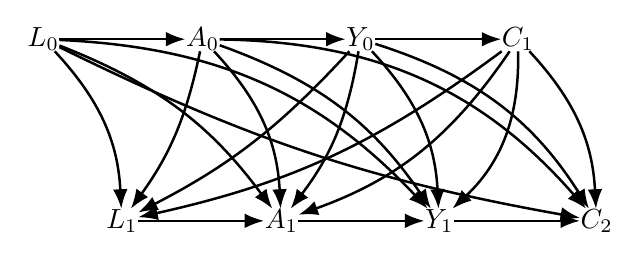
\begin{tikzpicture}[
  node distance = 1cm and 1.6cm,
  >=Latex, baseline,
  every node/.style={inner sep=0pt, anchor=center},
  main/.style={line width=0.9pt, draw=black},
  uniform/.style={line width=0.9pt, draw=black}
]
  % ----- time-0 nodes -----
  \node (L0) {$L_{0}$};
  \node[right=of L0] (A0) {$A_{0}$};
  \node[right=of A0] (Y0) {$Y_{0}$};
  \node[right=of Y0] (C1) {$C_{1}$};
  % ----- time-1 nodes (shifted right) -----
  \node[below=2cm of L0, xshift=1cm] (L1) {$L_{1}$};
  \node[right=of L1] (A1) {$A_{1}$};
  \node[right=of A1] (Y1) {$Y_{1}$};
  \node[right=of Y1] (C2) {$C_{2}$};
  % ----- within-time arrows (order inside each interval) -----
  \draw[->,uniform] (L0) -- (A0);
  \draw[->,uniform] (A0) -- (Y0);
  \draw[->,uniform] (Y0) -- (C1);
  \draw[->,uniform] (L1) -- (A1);
  \draw[->,uniform] (A1) -- (Y1);
  \draw[->,uniform] (Y1) -- (C2);
  % ----- cross-time "same-variable" persistence -----
  \draw[->,uniform,bend left=20] (L0) to (L1);
  \draw[->,uniform,bend left=20] (A0) to (A1);
  \draw[->,uniform,bend left=20] (Y0) to (Y1);
  \draw[->,uniform,bend left=20] (C1) to (C2);
  % ----- cross-time: all past → all future (now uniform black) -----
  % from L0
  \draw[->,uniform,bend left=16] (L0) to (A1);
  \draw[->,uniform,bend left=22] (L0) to (Y1);
  \draw[->,uniform,bend right=8] (L0) to (C2);
  % from A0
  \draw[->,uniform,bend left=12] (A0) to (L1);
  \draw[->,uniform,bend left=18] (A0) to (Y1);
  \draw[->,uniform,bend left=24] (A0) to (C2);
  % from Y0
  \draw[->,uniform,bend left=10] (Y0) to (L1);
  \draw[->,uniform,bend left=14] (Y0) to (A1);
  \draw[->,uniform,bend left=20] (Y0) to (C2);
  % from C1
  \draw[->,uniform,bend left=12] (C1) to (L1);
  \draw[->,uniform,bend left=18] (C1) to (A1);
  \draw[->,uniform,bend left=24] (C1) to (Y1);
\end{tikzpicture}
\caption{%
Causal diagram for a two-period longitudinal data structure illustrating time-varying
treatment, disease burden, censoring, and outcome processes. At each discrete time $t$,
the patient’s observed covariates $L_t$ summarize measured prognostic information
available prior to treatment assignment. Conditional on the history
$(\bar L_t, \bar A_{t-1})$, treatment $A_t$ is assigned by the clinical decision
process. Over the subsequent interval $(t,t+1]$, the patient may experience the outcome
$Y_{t+1}$ (e.g., death), may become censored $C_{t+1}$, and the disease process evolves
to $L_{t+1}$. Arrows indicate causal dependence across and within time periods,
including feedback between past treatment and future disease severity, motivating use
of the parametric g-formula.}
\label{fig:DAG2}
\end{figure}

\paragraph{Treatment strategies and estimands.}
A treatment strategy $g=(g_0,\ldots,g_K)$ is a deterministic dynamic rule that assigns
\[
a_t = g_t(\bar L_t,\bar a_{t-1}), \qquad t=0,\ldots,K.
\]
Under an intervention $g$, the treatment path $\bar a^g=(a_0^g,\ldots,a_K^g)$ is fixed
given the realized covariate history, even though the corresponding observed treatment
variables $\bar A$ are stochastic in observational data. Under the hypothetical
elimination of censoring, we write the counterfactual outcome at horizon $K+1$ as
\[
Y^g_{K+1} \equiv Y^{\bar a^g,\bar c=0}_{K+1}.
\]
Our goal is to compare risks under different strategies $g$ and $g'$ via contrasts such
as $\Pr(Y^g_{K+1}=1)-\Pr(Y^{g'}_{K+1}=1)$.

In our application, the primary strategy of interest $g$ is a closed-loop control policy
that mimics ICU titration of anti-seizure medication to maintain EA burden below a
target $\theta$ (Figure~\ref{fig:control-problem}D). A simple proportional--integral (PI)
policy can be written as
\begin{equation}
g_t(\bar L_t,\bar A_{t-1})
=
\min\!\left\{A_{\max},\,
\max\!\left\{0,\, \kappa_p e_t + \kappa_i \sum_{s=0}^{t} e_s \right\}\right\},
\qquad e_t = L_t-\theta,
\end{equation}
where $\kappa_p$ and $\kappa_i$ are proportional and integral gains and $A_{\max}$ is a
maximum safe dose. This closed-loop structure induces time-varying confounding: sicker
patients (higher $L_t$) tend to receive more treatment, while treatment affects future
$L_{t+1}$.

\subsection{Identification Assumptions}

Before using observational data to estimate causal effects, we specify assumptions under
which the counterfactual estimands are identifiable.

In plain language, three conditions must hold. (i) \emph{Sequential ignorability}: once we
condition on everything we have observed up to time $t$, the clinician's choice of dose at
$t$ and the chance of the patient leaving the study over the next interval are statistically
independent of what the patient's future survival would be under any given intervention.
This is an assumption about the \emph{assignment mechanism}, not a claim that treatment has
no effect. (ii) \emph{Positivity / overlap}: for histories that actually occur in the data,
the observed treatment and censoring mechanisms must have nonzero probability of producing
(or approaching, for continuous treatment) the action the intervention \(g\) would prescribe,
while the patient remains alive and uncensored. (iii) \emph{Consistency}: if the observed
treatment happens to match the intervention's prescription, the observed outcome equals the
counterfactual outcome under that intervention. Below we state these formally.

For each time $t=0,1,\ldots,K$, among individuals alive and uncensored at time $t$
(i.e., $\bar Y_t=\bar C_t=0$), we assume the following. Throughout, conditioning statements
are written in terms of $(\bar L_t,\bar A_{t-1})$; baseline covariates $X$ are fixed over
follow-up and are implicitly conditioned on in every such statement, so that the full
conditioning set is the observed history $H_t=(X,\bar L_t,\bar A_{t-1})$.

\textbf{(1) Sequential ignorability (no unmeasured confounding and no unmeasured informative censoring).}
Treatment and censoring behave ``as if randomized'' conditional on observed history:
\begin{equation}
\bigl(Y^g_{t+1},\ldots,Y^g_{K+1}\bigr)
\ \perp\!\!\!\perp\ 
\bigl(A_t, C_{t+1}\bigr)
\ \Bigm|\ 
\bar L_t=\bar l_t,\ \bar A_{t-1}=\bar a^g_{t-1},\ \bar C_t=\bar Y_t=0.
\end{equation}
This conditional independence concerns the assignment mechanisms for $A_t$ and
$C_{t+1}$, not the causal effect of treatment. It rules out unmeasured factors that,
given the observed history, jointly influence treatment decisions or censoring and the
future counterfactual outcomes under $g$.

\textbf{(2) Positivity (overlap).}
For histories that occur with positive density under the observed data-generating
process, there must be empirical support for the treatment levels prescribed by $g$
\emph{and} remaining uncensored. Because $A_t$ is continuous, we express positivity in
terms of neighborhoods. For each $k$ and each $\varepsilon>0$,
\begin{multline}
f_{\bar L_k,\bar A_{k-1},\bar C_k,\bar Y_k}\bigl(\bar l_k,\bar a_{k-1},0,0\bigr)>0
\ \Rightarrow\\
P\!\left(A_k \in \mathcal N_\varepsilon(a_k^g),\ C_{k+1}=0
\ \Bigm|\ \bar L_k=\bar l_k,\ \bar A_{k-1}=\bar a_{k-1},\ \bar C_k=\bar Y_k=0\right)>0,
\end{multline}
where $\mathcal N_\varepsilon(a)=\{a':|a'-a|<\varepsilon\}$ and
$a_k^g=g_k(\bar l_k,\bar a_{k-1})$. Intuitively, among histories that occur, the observed
data must contain nonzero probability of treatment values near those dictated by $g$,
while remaining alive and uncensored.

\textbf{(3) Consistency (well-defined interventions).}
If $\bar A_K=\bar a_K^g$ and $\bar C_{K+1}=0$, then $\bar L_K^g=\bar L_K$ and
$Y_{K+1}^g=Y_{K+1}$.

\subsubsection*{Plausibility of the positivity assumption}\label{sec:positivity}

Our target interventions are deterministic dynamic rules (closed-loop controllers) that
map histories to unique actions. In the extreme case where the observed treatment
mechanism followed a deterministic rule exactly, positivity would fail because for a
given history only one action would ever occur. In practice, ICU treatment exhibits
substantial stochastic variation across clinicians and time, including untreated
periods, intermittent dosing, and near--closed-loop titration. This heterogeneity
supports approximate overlap: within the range of histories observed, there is nonzero
probability of treatment values near those prescribed by reasonable target policies.

To further limit extrapolation, we restrict simulated interventions to operate within
empirically observed ranges of disease severity and dosing, thereby focusing estimation
on regions of the covariate--treatment space supported by the observed data.

Data generated according to the causal graph in Figure~\ref{fig:DAG2} satisfy these
identifiability conditions, as does the data-generating model considered in CICADAS.

\subsection{Identification via G-Formula for Causal Survival Analysis}

Under the above assumptions, the causal survival probability under policy $g$ is
identified by the parametric g-formula~\cite{robins1986new}. For our discrete-time survival outcome, the
probability of surviving through time $K+1$ under policy $g$ can be written as
\begin{align}
\label{eq:gformula_survival1}
P\bigl(Y^g_{K+1} = 0\bigr)
&= \sum_{\bar{l}_K}
\left[
\prod_{t=0}^{K}
P\Bigl(
Y_{t+1} = 0
\,\Bigm|\,
\bar{L}_t = \bar{l}_t,\,
\bar{A}_t = \bar{a}^g_t,\,
\bar{C}_t = \bar{Y}_t = 0
\Bigr)
\right]
f^g(\bar{l}_K),
\end{align}
where $f^g(\bar l_K)$ denotes the joint distribution of the covariate history $\bar L_K$
that would arise under policy $g$ under the hypothetical elimination of censoring (i.e.,
$\bar C=0$). Survival through time $K+1$ corresponds to the product over $t=0,\ldots,K$,
while the covariate history $\bar L_K$ is generated through transitions at
$t=0,\ldots,K-1$.

Although the estimand in \eqref{eq:gformula_survival1} is defined under elimination of
censoring, the observed data are subject to censoring. Assumption (1) is stated jointly
for treatment and censoring and therefore requires conditional independent censoring
given observed history; accordingly, we estimate the disease-evolution and outcome
models using only person-time during which individuals are alive and uncensored, without
fitting an explicit censoring model.

\paragraph{Simulating the covariate distribution under $g$.}
We do not estimate $f^g(\bar l_K)$ directly. Instead, we generate sample paths from it
by recursively simulating $L_{t+1}$ from the disease-evolution model
\[
f\bigl(L_{t+1}\mid \bar L_t,\bar A_t,\bar C_t=\bar Y_t=0\bigr)
\quad \text{with} \quad A_t = g_t(\bar L_t,\bar A_{t-1}),
\]
which yields trajectories distributed as $f^g(\bar L_K)$.
Under sequential ignorability and consistency, the conditional transition densities
under $g$ coincide with those estimable from observed data, giving the factorization
\[
f^g(\bar l_K)
=
\prod_{t=0}^{K-1}
f\!\left(
l_{t+1}
\,\middle|\,
\bar l_t,\,
\bar a_t^g,\,
\bar C_t=\bar Y_t=0
\right).
\]
A more detailed derivation is provided in Supplementary Section~S1.

\paragraph{Monte Carlo implementation.}
The summation in \eqref{eq:gformula_survival1} is generally intractable because it
requires integrating over all possible covariate trajectories. We therefore approximate
it by Monte Carlo simulation: generate $M$ sample paths
$\bar l_K^{(m)}=(l_0^{(m)},\ldots,l_K^{(m)})$ from the disease-evolution model under
policy $g$ (and $\bar C=0$), and compute
\begin{align}
P\bigl(Y^g_{K+1}=0\bigr)
&\approx
\frac{1}{M}\sum_{m=1}^{M}
\prod_{t=0}^{K}
P\Bigl(
Y_{t+1}=0
\,\Bigm|\,
\bar L_t=\bar l_t^{(m)},\,
\bar A_t=\bar a_t^g,\,
\bar C_t=\bar Y_t=0
\Bigr),
\end{align}
where $\bar l_t^{(m)}=(l_0^{(m)},\ldots,l_t^{(m)})$ is the covariate history along the
$m$-th simulated trajectory.

\paragraph{Models required for implementation.}
Implementing the Monte Carlo g-formula requires estimating two statistical models from
the observed (uncensored) data:
\begin{enumerate}
\item \textbf{Disease evolution model:}
\[
f\!\left(L_{t+1}\mid \bar L_t,\bar A_t,\bar C_t=\bar Y_t=0\right).
\]
\item \textbf{Outcome (mortality) model:}
\[
P\!\left(Y_{t+1}=1\mid \bar L_t,\bar A_t,\bar C_t=\bar Y_t=0\right).
\]
\end{enumerate}

\paragraph{Relation to alternative g-formula estimators.}
A comparison of the Monte Carlo parametric g-formula used here with iterated-conditional-expectation
and weighting-based alternatives is given in Supplementary Section~S1.3.

\section{The CICADAS Simulation Model}
\label{sec:datagen}
Sections~4 and~5 together specify and estimate the two model components required by the parametric g-formula introduced in Section~3.3: (i) the disease-evolution model for
$L_{t+1} \mid \bar{L}_t, \bar{A}_t$, and (ii) the discrete-time hazard model for
$Y_{t+1} \mid \bar{L}_t, \bar{A}_t$.
We present these components in a mechanistic and sequential manner that mirrors ICU physiology and clinical decision-making, and that ensures parameter identifiability before counterfactual trial emulation.

\paragraph{Roadmap.} The full simulated data-generating mechanism has five interlocking
pieces, each tied to a concrete clinical question:
(i) the \emph{disease-dynamics model} (Sec.~4.1) describes how
epileptiform-activity burden $L_{0,t}$ would evolve in the absence of treatment, capturing
the early rise, peak, and gradual resolution seen clinically;
(ii) the \emph{pharmacokinetic--pharmacodynamic (PKPD) model} (Sec.~4.2) tracks drug
concentration in a one-compartment approximation and maps it to the multiplicative
suppression of disease burden, with patient-specific potency and steepness modulated by age
and SOFA;
(iii) the \emph{outcome (mortality) hazard model} (Sec.~4.3) gives the discrete-time
probability of death as a function of cumulative disease and treatment burden;
(iv) the \emph{censoring model} (Sec.~4.4) generates informative loss-to-follow-up that
depends on treatment status; and
(v) the \emph{treatment-assignment model} (Sec.~4.5) generates two parallel cohorts---an
idealized RCT and a realistically confounded observational dataset.
Only components (i) and (iii) are strictly required as inputs for the g-formula in applied
settings; (ii), (iv), and (v) are used here to construct a realistic simulation with known
ground truth.

In this present section, we present our realistic synthetic data generation procedure. To simulate this system, we specify parametric models for disease progression, treatment effect, and patient outcome. Time is discretized into 2-hour intervals over a 7-day (168-hour) horizon.

\subsection{Disease Dynamics Model}
\label{sec:disease_dynamics}

In our system, the underlying disease intensity in the absence of treatment, $L_{0,t}$, is modeled as a stochastic process that captures three clinically motivated features of ICU epileptiform activity: (i) an early phase of rapid escalation, (ii) saturation at a characteristic peak intensity, and (iii) a later phase of gradual spontaneous resolution with decreasing variability. The evolution of $L_{0,t}$ is given by
\begin{equation}
\label{eq:disease_evolution}
L_{0,t+\Delta t}
=
\Big(
L_{0,t}
+ \mu(L_{0,t}, t)\,\Delta t
+ \sigma(L_{0,t}, t)\,\sqrt{\Delta t}\,Z
\Big)_+,
\end{equation}
where $Z \sim \mathcal{N}(0,1)$, $(x)_+ = \max(x,0)$ enforces nonnegativity of disease burden, $\mu(\cdot)$ is the deterministic drift term, and $\sigma(\cdot)$ controls stochastic variability.

The drift term $\mu(L_{0,t}, t)$ is defined in terms of a characteristic disease intensity scale $H$, which represents the typical peak (or carrying-capacity–like) level of epileptiform activity observed in critically ill patients:
\begin{equation}
\label{eq:disease_drift}
\mu(L_{0,t}, t)
=
\begin{cases}
h\,L_{0,t}\!\left(1 - \dfrac{L_{0,t}}{H}\right)
\;-\;
\alpha \max(0, L_{0,t} - H),
& t < 30, \\[8pt]
-\alpha\!\left(L_{0,t} - 0.2\,H e^{-\delta (t-30)}\right)
\;-\;
\alpha \max(0, L_{0,t} - H),
& t \ge 30 .
\end{cases}
\end{equation}

For early times ($t<30$ hours), the first term implements logistic-like growth: disease intensity initially increases approximately exponentially when $L_{0,t} \ll H$, but the growth rate diminishes as $L_{0,t}$ approaches $H$, preventing unbounded escalation. The additional penalty term $-\alpha \max(0, L_{0,t}-H)$ introduces stronger downward pressure when disease intensity exceeds the characteristic peak, producing a soft upper bound rather than a hard cutoff.

For later times ($t \ge 30$ hours), the drift switches to a mean-reverting form that models spontaneous recovery. In this phase, disease intensity is pulled toward a decaying baseline $0.2\,H e^{-\delta (t-30)}$, representing gradual resolution of the underlying pathological process. The same overshoot penalty is retained to discourage unrealistically persistent disease levels above $H$. Together, these components produce trajectories that rise, peak, and then resolve over clinically plausible time scales.

Stochastic variability is governed by the diffusion term
\begin{equation}
\label{eq:disease_diffusion}
\sigma(L_{0,t}, t)
=
\big[ \sigma_{\mathrm{early}} e^{-t/\tau}
+ \sigma_{\mathrm{late}} \big]
\sqrt{\max(0.001, L_{0,t})}.
\end{equation}
which allows higher volatility early in the course of illness and progressively stabilizes over time. The square-root dependence on $L_{0,t}$ ensures that variability scales with disease burden while remaining well-defined near zero.

Together, Equations~\eqref{eq:disease_evolution}--\eqref{eq:disease_diffusion}
generate disease trajectories that rise, peak, and resolve over clinically
plausible time scales, providing the natural-history component of the
CICADAS data-generating process. This behavior is consistent with empirically observed patterns of epileptiform activity in critically ill patients and provides a realistic substrate for evaluating time-varying treatment and outcome models within the CICADAS framework. Examples of disease natural-history trajectories generated by this model are shown in Figures~\ref{fig:control-problem} and~\ref{fig:swimmer_survival_rct}.

\subsection{Pharmacokinetic-Pharmacodynamic (PKPD) Model}
\label{sec:pkpd_model}
We leverage standard PKPD models to model the treatment effect~\cite{sheiner1979simultaneous,gabrielsson2016pharmacokinetic,hughes1992context}. We approximate the drug concentration in the body $x_t$ over time under treatment using a one-compartment pharmacokinetic model:
\begin{equation}
x_t = k_e x_{t-1} + A_t
\end{equation}
where $k_e$ is an elimination constant and $A_t$ is the drug dose administered. The pharmacodynamic effect $s_{x_t}$ is a reverse sigmoid function of the concentration $x_t$:
\begin{equation}
s_{x_t} = 1 - \frac{1}{(C_{50}/x_t)^\gamma + 1},
\end{equation}
such that $s_{x_t}$ decreases from 1 to 0 as drug concentration $x_t$ increases. The patient-specific parameters $C_{50}$ (concentration for 50\% effect) and $\gamma$ (Hill coefficient) depend on baseline covariates, allowing for heterogeneous treatment responses (see below). The observed disease intensity is the product of the underlying disease and the drug effect:
\begin{equation}
L_t = L_{0,t} \cdot s_{x_t}
\end{equation}

\paragraph{Population heterogeneity (mixed effects).}
We model patient-specific pharmacodynamics, the $C_{50}$ and Hill coefficient heterogeneity with baseline covariates via mixed effects. For illustration, consider just two baseline covariates, age and Sequential Organ Failure Assessment (SOFA) score:
\begin{align}
C_{50,i} &= \beta^C_0 + \beta^C_1 \cdot \mathrm{age}_i^* + \beta^C_2 \cdot \mathrm{SOFA}_i^* + \eta^C_i, \\
\gamma_i &= \beta^\gamma_0 + \beta^\gamma_1 \cdot \mathrm{age}_i^* + \beta^\gamma_2 \cdot \mathrm{SOFA}_i^* + \eta^\gamma_i,
\end{align}
where $z^* = (z - \bar z)/\sigma_z$ denotes standardization, and $\eta^C_i \sim \mathcal{N}(0,\sigma_C^2)$, $\eta^\gamma_i \sim \mathcal{N}(0,\sigma_\gamma^2)$ are patient-level random effects.

\subsection{Outcome Model}
\label{sec:outcome-model}
\label{subsec:death_model}
We model mortality using a discrete-time hazard function $h_{i,t}$, defined as the probability of death for patient $i$ during interval $(t,t+1]$, conditional on being alive and uncensored up to time $t$:
\[
h_{i,t}
= P\!\left(
Y_{i,t+1} = 1
\;\middle|\;
\bar{Y}_{i,t} = 0,\;
\bar{C}_{i,t} = 0,\;
\bar{L}_{i,t},\;
\bar{A}_{i,t}
\right).
\]
The logit of the hazard depends on baseline time effects and cumulative harm from both disease and treatment, with susceptibility modified by patient characteristics:
\begin{equation}
\text{logit}\,h_{i,t} 
= \alpha_0 
+ \alpha_1 \left( \frac{t}{T_{\max}} \right)^2
+ (\alpha_2 + \alpha_3 \cdot \mathrm{SOFA}_i) \left( \frac{\sum_{s=0}^t L_{i,s}}{L_{\mathrm{norm}}} \right)^2
+ (\alpha_4 + \alpha_5 \cdot \tfrac{\mathrm{Age}_i}{\mathrm{Age}_{\mathrm{norm}}}) \left( \frac{\sum_{s=0}^t A_{i,s}}{A_{\mathrm{norm}}} \right).
\label{eq:death_model}
\end{equation}
Here:
\begin{itemize}
    \item \(T_{\max}\) scales time (e.g., 170 h) to stabilize estimation.
    \item \(L_{\mathrm{norm}}\) (e.g., 24 units) normalizes cumulative disease burden.
    \item \(A_{\mathrm{norm}}\) (e.g., 207 units) normalizes cumulative treatment exposure.
    \item \(\mathrm{SOFA}_i\) and \(\mathrm{Age}_i\) are baseline patient covariates (included in the vector of baseline covariates \(L_{i,0}\) in the g-formula framework).
\end{itemize}
This structure captures: (i) a smooth baseline time effect, (ii) accumulation of disease-related harm, 
(iii) accumulation of treatment-related harm, and (iv) effect modification by baseline patient characteristics 
(critical illness severity, measured by SOFA score, and age). 
Although this functional form omits potential \textit{direct} effects of SOFA or age on mortality beyond their interaction 
with cumulative burden, it is intended only as a stylized data-generating process for simulation rather than as 
a clinically validated model. In practice, more flexible outcome models could include independent main effects of 
SOFA or age without altering the causal inference framework.

\subsection{Censoring Model}
\label{subsec:censoring_model}
Loss to follow-up in the simulated observational cohort is generated by a discrete-time hazard that
depends on treatment status, accumulated treatment burden, accumulated disease burden, and elapsed
time. Censoring is therefore \emph{informative}: it depends on the same quantities that drive
mortality, so ignoring it biases naive analyses. No censoring is applied in the randomized cohort,
which is what allows that cohort to serve as an unmodeled ground truth.

equation

The censoring model is used only to construct a realistic observational cohort; it is not required
as an input to the g-formula in applied settings, where the censoring mechanism must instead be
estimated from the data. Section~\ref{sec:robustness} reports how the estimator behaves when the
censoring mechanism departs from the one assumed. Full parameterization is given in Supplementary
Section~S2.2.

\subsection{Treatment Assignment Model}
\label{sec:TreatmentAssignment}
Two cohorts are generated from identical disease and PK/PD models, differing only in how treatment is
assigned. In the \emph{randomized} cohort, each patient is assigned to closed-loop control or to no
treatment with probability one-half, independently of all patient characteristics. In the
\emph{observational} cohort, the probability of treatment is an increasing function of early disease
burden, SOFA score, and the trajectory's early slope and acceleration, so that sicker and
faster-deteriorating patients are preferentially treated.

equation

This is the mechanism that generates confounding by indication: because treatment probability depends
on early severity, and early severity predicts death, the treated group is sicker at baseline and
treatment appears less beneficial than it is. Section~\ref{sec:cohorts} quantifies the resulting bias
over 400 replications. Full parameterization is given in Supplementary Section~S2.3.

\subsection{Model Parameters}
The full set of model variables, their symbols, units, and the ground-truth values used to generate
the synthetic cohorts is given in Supplementary Table~S1. Section~\ref{sec:estimation} describes how
each component is estimated from data; Section~\ref{sec:results} reports how accurately the
generating values are recovered.

%========================================================
\section{Estimation of Model Parameters}
\label{sec:estimation}
%========================================================
This section describes the estimation framework used in CICADAS. The goal is to construct a fully
specified generative model for disease burden, treatment effects, and mortality that can serve as the
kernel of the parametric g-formula. Full derivations, filter recursions, and implementation details
are given in the Supplementary Material; what follows is the logic of the procedure.

\paragraph{Plain-English preview.} The estimation problem has three pieces. \emph{First}, we use
untreated patients to learn how epileptiform activity evolves on its own (the disease-dynamics
parameters). Because untreated patients receive no drug, the observed severity trajectory is a direct
read-off of the underlying disease process. \emph{Second}, we use patients whose dose changes during
the ICU stay to learn how the drug affects severity (the PK/PD parameters). These patients provide
enough variation in exposure to separate the drug's effect from the background disease dynamics;
patients on constant closed-loop control do not. \emph{Third}, we use the full cohort to learn how
cumulative disease burden and cumulative treatment burden combine into a death hazard (the outcome
parameters). Once these three components are fitted, we simulate counterfactual trials under
alternative dosing policies by forward Monte Carlo from the fitted generative model and compare the
resulting survival curves---this is the g-formula in operation.

%--------------------------------------------------------
\subsection{Overview}
%--------------------------------------------------------
CICADAS proceeds in two phases. \textbf{Phase 1 (model estimation)} constructs the generative model by
estimating its components from observed data, in three stages: disease natural history, PK/PD
parameters, and the mortality hazard. \textbf{Phase 2 (trial emulation)} applies the parametric
g-formula to the fitted model, simulating counterfactual outcomes for the whole cohort under
alternative dynamic treatment strategies and producing counterfactual survival curves and policy
contrasts. Figure~\ref{fig:pipeline} shows the full workflow.

When CICADAS is applied to real ICU data, Phase~2 is the causal effect estimator. In this paper, where
all data are simulated, we additionally generate synthetic datasets from a known data-generating
process and reapply the same trial emulation to assess whether it recovers the causal effects that are
true by construction (Section~\ref{ssec:validation-framework}).

\begin{figure}[htbp]
\centering
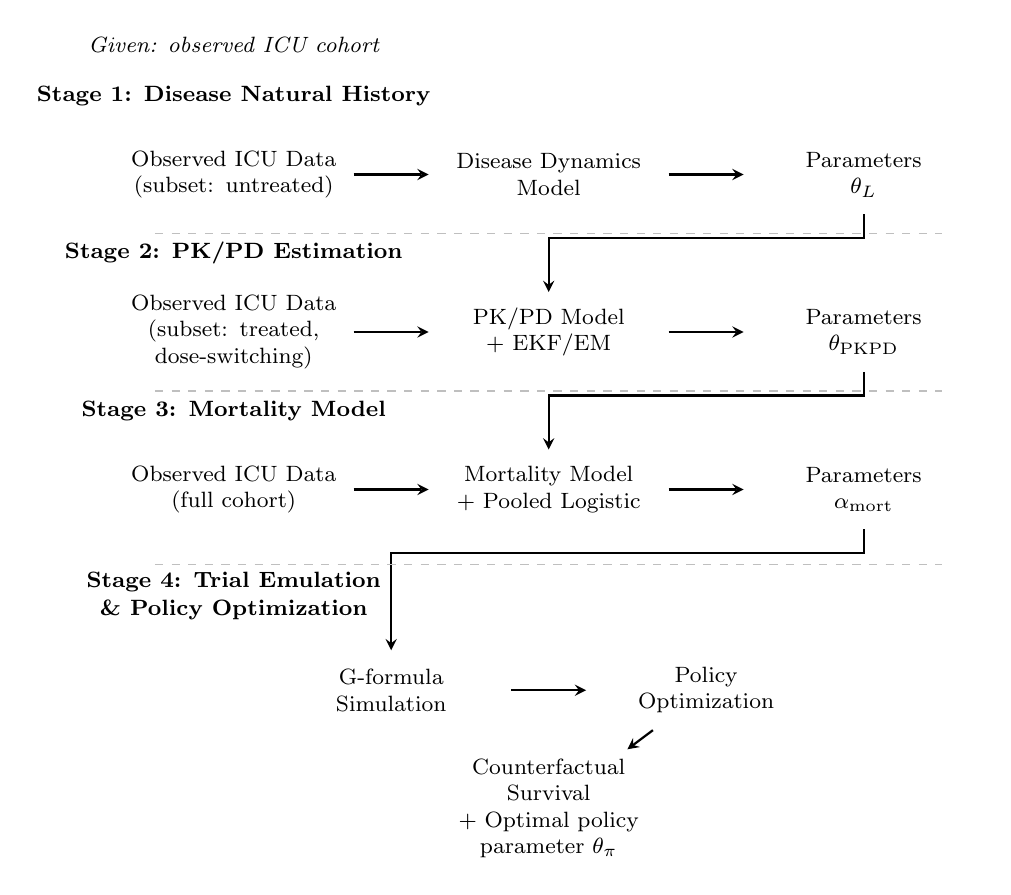
\begin{tikzpicture}[
    node distance=1.5cm and 3cm,
    component/.style={text width=2.8cm, text centered, minimum height=1cm, font=\footnotesize},
    arrow/.style={->, >=stealth, thick, black},
    stage/.style={font=\bfseries\footnotesize},
    note/.style={font=\footnotesize\itshape, text centered}
]

% Starting point (centered over Stage 1 left node)
\node[note] at (0,8.15) {Given: observed ICU cohort};

% Stage titles
\node[stage] at (0,7.5) {Stage 1: Disease Natural History};
\node[stage] at (0,5.5) {Stage 2: PK/PD Estimation};
\node[stage] at (0,3.5) {Stage 3: Mortality Model};
\node[stage] at (0,1.15) {\shortstack{Stage 4: Trial Emulation\\\& Policy Optimization}};


% Stage 1
\node[component] (raw_data1)     at (0,6.5) {Observed ICU Data\\(subset: untreated)};
\node[component] (disease_model) at (4,6.5) {Disease Dynamics\\Model};
\node[component] (disease_params)at (8,6.5) {Parameters\\$\theta_L$};

% Stage 2
\node[component] (raw_data2)     at (0,4.5) {Observed ICU Data\\(subset: treated, dose-switching)};
\node[component] (pkpd_model)    at (4,4.5) {PK/PD Model\\+ EKF/EM};
\node[component] (pkpd_params)   at (8,4.5) {Parameters\\$\theta_{\mathrm{PKPD}}$};

% Stage 3
\node[component] (raw_data3)     at (0,2.5) {Observed ICU Data\\(full cohort)};
\node[component] (mortality_model)at (4,2.5) {Mortality Model\\+ Pooled Logistic};
\node[component] (mortality_params)at (8,2.5) {Parameters\\$\alpha_{\mathrm{mort}}$};

% Stage 4 (moved DOWN slightly for breathing room)
\node[component] (gformula)      at (2,-0.05) {G-formula\\Simulation};
\node[component] (optimization)  at (6,-0.05) {Policy\\Optimization};
\node[component] (survival_curves)at (4,-1.55) {Counterfactual Survival\\+ Optimal policy\\parameter $\theta_{\pi}$};

% Horizontal arrows within stages
\draw[arrow] (raw_data1) -- (disease_model);
\draw[arrow] (disease_model) -- (disease_params);

\draw[arrow] (raw_data2) -- (pkpd_model);
\draw[arrow] (pkpd_model) -- (pkpd_params);

\draw[arrow] (raw_data3) -- (mortality_model);
\draw[arrow] (mortality_model) -- (mortality_params);

\draw[arrow] (gformula) -- (optimization);

% Right-angle arrows between stages (shorter drop to reduce clutter near dashed lines)
\draw[arrow] (disease_params.south) -- +(0,-0.30) -| (pkpd_model.north);
\draw[arrow] (pkpd_params.south) -- +(0,-0.30) -| (mortality_model.north);
\draw[arrow] (mortality_params.south) -- +(0,-0.30) -| (gformula.north);

% Final output arrow
\draw[arrow] (optimization) -- (survival_curves);

% Stage separation lines (nudged to avoid Stage 4 title/arrow crowding)
\draw[gray!50, dashed] (-1,5.75) -- (9,5.75);
\draw[gray!50, dashed] (-1,3.75) -- (9,3.75);
\draw[gray!50, dashed] (-1,1.55) -- (9,1.55);

\end{tikzpicture}
\caption{CICADAS workflow applied to observed ICU data. Stage~1 fits the disease natural-history model using untreated patients, Stage~2 fits PK/PD parameters using treated patients with dose switching, and Stage~3 fits the mortality model using the full cohort, yielding $\theta_L$, $\theta_{\mathrm{PKPD}}$, and $\alpha_{\mathrm{mort}}$. Stage~4 uses these fitted components within the parametric g-formula to emulate counterfactual trials under candidate dynamic treatment policies and to optimize a policy parameter $\theta_{\pi}$.}
\label{fig:pipeline}
\end{figure}

\subsection{Data Structure}
Estimation operates on person-time (long) format: one row per patient per time interval, recording
severity $L_t$, treatment intensity $A_t$, censoring and death indicators, and baseline covariates.
An example is given in Supplementary Table~S2.

\subsection{Step 1: Disease Natural History}
The natural-history parameters $\theta_L$ govern how epileptiform-activity burden would evolve absent
treatment. They are estimated from untreated patients, for whom $L_t = L_{0,t}$ by definition, so that
the observed trajectory identifies the underlying process directly without needing to disentangle a
drug effect. We fit the growth, peak, decay, and volatility parameters of the stochastic
disease-dynamics model of Section~\ref{sec:disease_dynamics} by maximum likelihood over the observed
trajectories. Using untreated patients for this step is what makes the subsequent PK/PD step
identifiable: with the background process pinned down, the residual suppression observed in treated
patients is attributable to drug exposure.

\subsection{Step 2: PK/PD Parameter Estimation}
The PK/PD parameters map treatment intensity to suppression of disease burden. Drug concentration is
unobserved, so the model is a nonlinear state-space system: a latent one-compartment concentration
driven by the observed infusion rate, mapped through a Hill function to multiplicative suppression of
the natural history, with patient-specific potency $C_{50}$ and steepness $\gamma$ modeled as
mixed effects on age and SOFA score.

\paragraph{Why dose-switching observational data are required.}
Identification of $(C_{50},\gamma)$ requires variation in exposure within a patient. A patient held at
a stable dose under effective closed-loop control provides almost no information about the shape of
the dose--response curve, because the observed severity is nearly constant and the concentration
occupies a narrow range. Patients whose dose changes during the stay---because of sedation
interruptions, escalation, or weaning---sweep out a range of concentrations and therefore identify the
curve. This is a substantive design requirement, not a technical convenience: it means the framework
depends on precisely the practice variation described in Section~\ref{sec:clinical-problem}, and a
uniformly protocolized cohort would be uninformative for this step.

\subsubsection*{Estimation procedure}
We fit the state-space model by expectation--maximization, using an extended Kalman filter with a
Rauch--Tung--Striebel smoother for the E-step and closed-form updates for the M-step. The full
recursions, the four alternative estimation strategies we compared (joint estimation, oracle $k_e$,
raw two-stage, and two-stage with bias correction), the design diagnostics used to screen patients for
inclusion, uncertainty quantification, and implementation details are given in Supplementary
Section~S3.

The practically important result, reported in Section~\ref{sec:pkpd-results}, is that the two-stage
estimator with bias correction approaches oracle accuracy without requiring the elimination constant
$k_e$ to be known in advance, whereas joint estimation over all parameters simultaneously is unstable
in the presence of parameter interactions and local optima.

\subsection{Step 3: Mortality Model}
The outcome model is a discrete-time hazard fitted by pooled logistic regression on the full cohort,
in which the log-odds of death in each interval depend on cumulative disease burden, cumulative drug
exposure, elapsed time, and baseline severity, with the disease and drug terms scaled by SOFA score and
age respectively. Pooled logistic regression is used because it approximates the discrete-time hazard
directly and extends naturally to the time-varying covariates that the g-formula must simulate forward.
The fitted hazard, together with the disease and PK/PD components, completes the generative model
required by the g-formula.

\subsection{Design Diagnostics}\label{sec:design_diagnostics}
Before any causal estimate is produced, we recommend reporting a set of design diagnostics that
establish whether the data can support the intended policy comparison: the distribution of dose
conditional on severity, the proportion of person-time spent in a concentration range that identifies
the dose--response curve, the observed range of achieved severity relative to the policy thresholds
being evaluated, and the fraction of person-time censored together with the covariates predicting
censoring. The full set is given in Supplementary Table~S3, and Section~\ref{sec:conditions} states
how each maps onto a precondition for applying the framework to real data.

\subsection{Validating the G-Formula Estimator in Simulation}\label{ssec:validation-framework}
Because all data in this paper are simulated, the causal effect of each policy is known by
construction, which allows a direct test of whether the estimator recovers it. We generate two
parallel cohorts from the same disease and PK/PD models, differing only in the treatment-assignment
mechanism: a randomized cohort, in which assignment is independent of patient characteristics and no
censoring occurs, and an observational cohort, in which sicker patients are preferentially treated and
censoring is informative. The randomized cohort supplies the ground truth, obtained directly as the
difference in survival proportions with no modeling. The estimator is then applied to the
observational cohort alone and its output compared with that ground truth.

Performance is assessed on three criteria: bias of the estimated policy contrast against the ground
truth at 168 hours; coverage of bootstrap confidence intervals; and agreement between the estimated
and true counterfactual survival curves over the whole follow-up rather than at the endpoint alone. We
report the same comparison for naive Kaplan--Meier, stabilized IPTW, and a marginal structural model,
so that the g-formula's performance can be read against alternatives applied to identical data.

\subsection{Sensitivity analyses and benchmarking}\label{sec:sensitivity}

To evaluate the robustness of the CICADAS g-formula to violations of its identification
assumptions and to compare it against alternative causal-inference estimators, we ran four
additional experiments on the simulated observational cohort. Code for all four is provided
in the \texttt{sensitivity/} and \texttt{benchmarks/} subdirectories of the public
repository.

\paragraph{Unmeasured confounding (NUC injection).}
We modified the data-generating process to include a binary confounder
\(U \sim \mathrm{Bernoulli}(0.5)\) that is observed by the clinician but hidden from the
estimator: it shifts the treatment-assignment logit by \(\delta_A\) and the mortality
hazard logit by \(\delta_Y\). For each combination on a \(5 \times 5\) grid of
\((\delta_A, \delta_Y) \in \{0, 0.5, 1.0, 1.5, 2.0\}^2\), we generated 3 cohorts of
\(N = 1500\) patients, ran the full CICADAS g-formula pipeline without access to \(U\),
and recorded the resulting bias in the recovered ATE relative to the oracle RCT ATE that
also experiences \(U\). We additionally computed the Ding--VanderWeele E-value~\cite{vanderweele2017evalue} for the
honest ATE (\(\delta_A = \delta_Y = 0\)) and identified the smallest \(\delta_Y\) at
\(\delta_A = 0\) at which the g-formula ATE changes sign.

\paragraph{Measurement error on the EEG-severity proxy.}
We added independent Gaussian noise with standard deviation \(\sigma \in
\{0, 0.01, 0.025, 0.05, 0.1, 0.2\}\) to each observed value of \(L_t\), clipped at zero,
and re-ran the g-formula pipeline on the perturbed data.

\paragraph{Alternative censoring mechanisms.}
We replaced the baseline treatment-dependent informative censoring with three alternatives:
(i) missing completely at random (flat low rate, independent of covariates);
(ii) strongly outcome-dependent censoring (amplified coefficients on cumulative disease
and treatment burden); and (iii) no censoring at all. We compared recovered ATEs across
regimes.

\paragraph{Benchmarking against alternative estimators.}
We compared the CICADAS g-formula against two alternative causal-inference estimators:
(a) stabilized inverse probability of treatment weighting (IPTW)~\cite{robins2000marginal,cole2008constructing} using a pooled logistic
propensity model on the baseline covariates (age, SOFA, early-phase disease severity);
(b) a marginal structural model (MSM)~\cite{robins2000marginal,hernan2000marginal} fit as a weighted pooled logistic regression for
the discrete-time mortality hazard on time and treatment, using the IPTW weights.
We also report a naive Kaplan--Meier estimate from the same observational data as a
reference for the magnitude of confounding. Targeted minimum-loss estimation (TMLE)~\cite{vanderlaan2006tmle,vanderlaan2011targeted} is
not included here as a direct comparator because established implementations
(\texttt{ltmle}, \texttt{survtmle})~\cite{lendle2017ltmle,benkeser2017survtmle} are in R and including them would introduce a
non-trivial cross-language dependency; we discuss this in Section~7 as a direction for
follow-up work. 95\% confidence intervals for IPTW, MSM, and the naive KM estimator come
from 200-replicate nonparametric subject-level bootstrap; the g-formula CIs use the
1000-replicate bootstrap described earlier in this section.

\section{Simulation Study: Internal Validation and Benchmarking}
\label{sec:results}

\subsection{Simulation Setup and Ground-Truth Parameters}

We generated a \textit{synthetic ICU dataset} for patients observed over 168 hours. For PKPD estimation experiments, we used $N=1000$ patients treated with the stochastic, stepwise dose-switching treatment pattern. For all other experiments, we simulated $N=2000$ subjects treated with either closed-loop control or no treatment, with probabilities of being assigned to each group either uniformly random when simulating a true RCT, or assigned as described in Section~\ref{sec:TreatmentAssignment} when simulating observational data.


\subsection{Simulated Cohorts and the Confounding Problem}
\label{sec:cohorts}

All results in this section are obtained from synthetic cohorts generated by the model of
Section~\ref{sec:datagen}, in which the true causal effect of each policy is known by construction.
We generated two parallel cohorts of $N = 2000$ patients each over a 168-hour horizon, differing only
in how treatment was assigned. In the \textbf{simulated trial} cohort, patients were assigned to
closed-loop control at $\theta = 0.1$ or to no treatment with equal probability, independently of
patient characteristics. In the \textbf{simulated observational} cohort, assignment followed the
confounded mechanism of Section~\ref{sec:TreatmentAssignment}, in which sicker patients are
preferentially treated, and informative censoring was applied. A separate cohort of $N = 1000$
patients receiving stochastic stepwise dose-switching was generated for the PK/PD estimation
experiments of Section~\ref{sec:pkpd-results}.

Because assignment in the trial cohort is randomized and that cohort is uncensored, the difference in
168-hour survival between its arms requires no modeling: it is obtained directly as the difference in
the proportion surviving. This quantity is the ground truth of the simulation, and it is the benchmark
against which every observational estimator below is measured.

\paragraph{Monte Carlo replication of the confounding effect.}
Because a single simulated cohort gives only one draw from the data-generating process, we replicated
the entire generation-and-analysis procedure over 400 independent replications (200 seeds in each of
the MATLAB and Python implementations, $N = 2000$ per cohort). Table~\ref{tab:multiseed} reports the
resulting sampling distributions. The ground-truth policy contrast averaged $+14.6$ percentage points
(Monte Carlo SE $0.11$), and naive Kaplan--Meier analysis of the confounded cohort averaged $+1.0$
points (MCSE $0.16$): confounding by indication eliminated 93\% of the true treatment effect. In
39\% of replications the attenuation was severe enough to reverse the sign of the estimate, so that
naive analysis indicated net harm from a treatment that was in fact beneficial. The two independent
implementations agreed on all three quantities to within Monte Carlo error (Welch $p \geq 0.06$;
two-sample Kolmogorov--Smirnov $p \geq 0.11$).

We report these as distributions rather than as a single cohort's values deliberately. Sign reversal
is a property of a substantial minority of replications, not of the data-generating process as such,
and the stable and more informative characterization of the confounding in this simulation is the
93\% attenuation of the true effect. All figures in this section display one representative cohort;
the quantities that carry the paper's claims are the replicated estimates in
Table~\ref{tab:multiseed}.

\begin{table}[htbp]
\centering
\begin{tabular}{lrrrr}
\toprule
Quantity & Mean & SD & MCSE & 95\% range \\
\midrule
Ground-truth ATE (randomized cohort)   & $+14.57$ & $2.17$ & $0.109$ & $[+10.81, +18.70]$ \\
Naive Kaplan--Meier ATE (observational) & $+1.00$  & $3.12$ & $0.156$ & $[-5.33, +6.90]$ \\
Bias of the naive estimator             & $-13.57$ & $3.79$ & $0.189$ & $[-21.24, -6.52]$ \\
\bottomrule
\end{tabular}
\caption{Sampling distribution of the ground-truth and naive treatment effects over 400 independent
simulated replications (200 seeds each in the MATLAB and Python implementations; $N=2000$ per cohort;
168-hour endpoint). All values are percentage points. The naive estimator retains 7\% of the true
effect on average and reverses its sign in 156/400 (39\%) of replications. All data are simulated.}
\label{tab:multiseed}
\end{table}

Figure~\ref{fig:swimmer_survival_rct} illustrates one representative pair of cohorts. In the trial cohort, the similar early coloring of the two arms in the
disease-burden heatmap reflects successful randomization: treated and untreated patients begin with
comparable severity. The untreated natural history is monophasic, rising rapidly and then tapering,
and although the disease eventually resolves without treatment, many patients die first. Treatment
intensity is highest where disease intensity is highest, reflecting the closed-loop policy, and the
clean separation between arms reflects perfect adherence and no dropout. In the observational cohort,
the treated group is visibly more severe from the outset, because clinicians in that cohort
preferentially treat sicker patients. The consequence is the central difficulty this paper addresses:
patients most likely to benefit from treatment are also most likely to die regardless of it, so
treatment appears harmful or ineffective under naive analysis.

\begin{figure}[htbp]
   \centering
   \noindent\textbf{(A) Simulated randomized trial}\par\vspace{0.2em}
   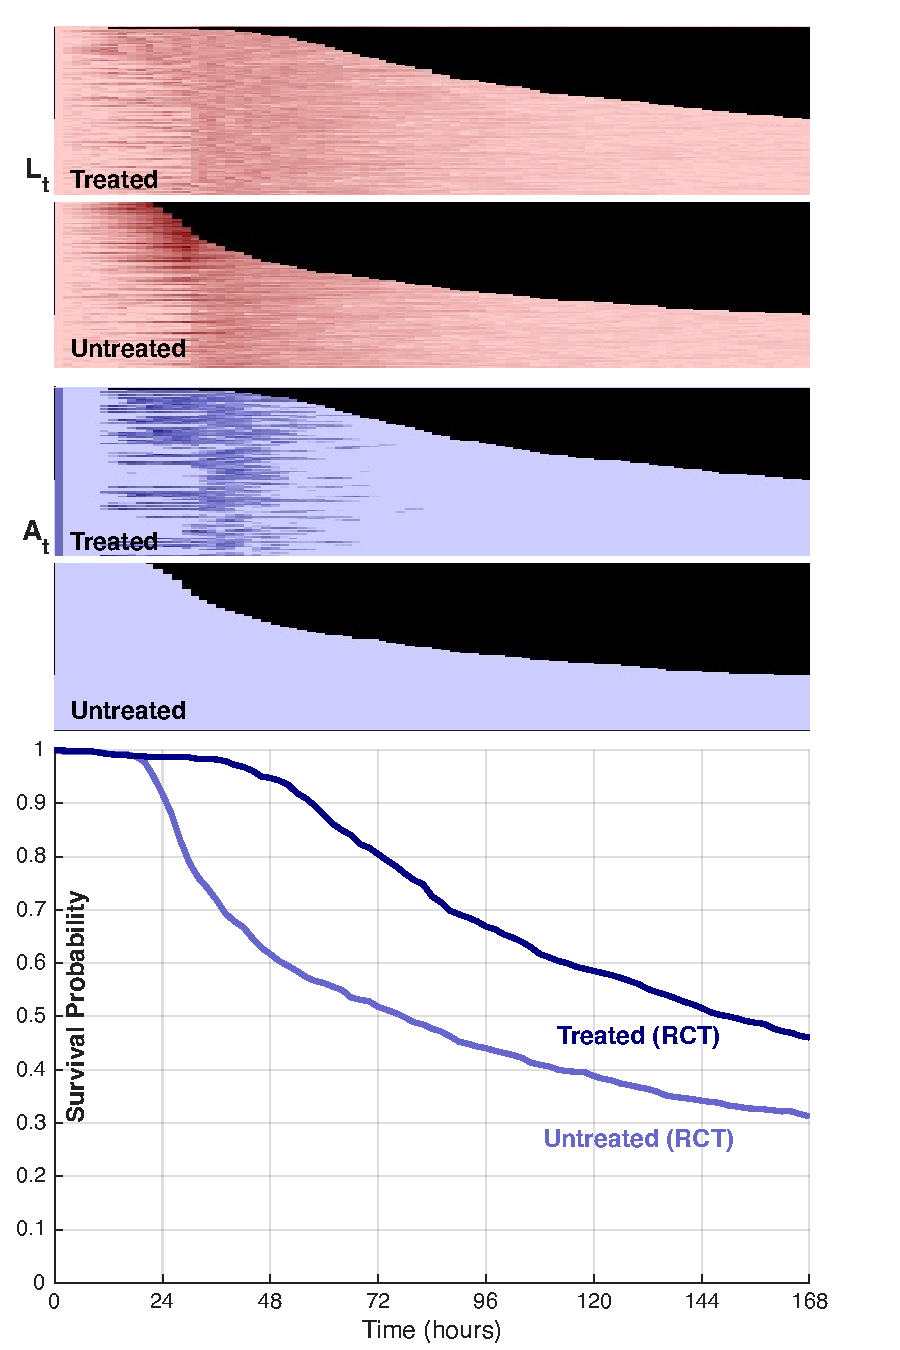
\includegraphics[width=0.68\textwidth,height=0.38\textheight,keepaspectratio, trim = 5pt 0pt 5pt 5pt, clip]{Fig3_swimmer_survival_plot_RCT.pdf}

   \vspace{0.9em}

   \noindent\textbf{(B) Simulated observational cohort}\par\vspace{0.2em}
   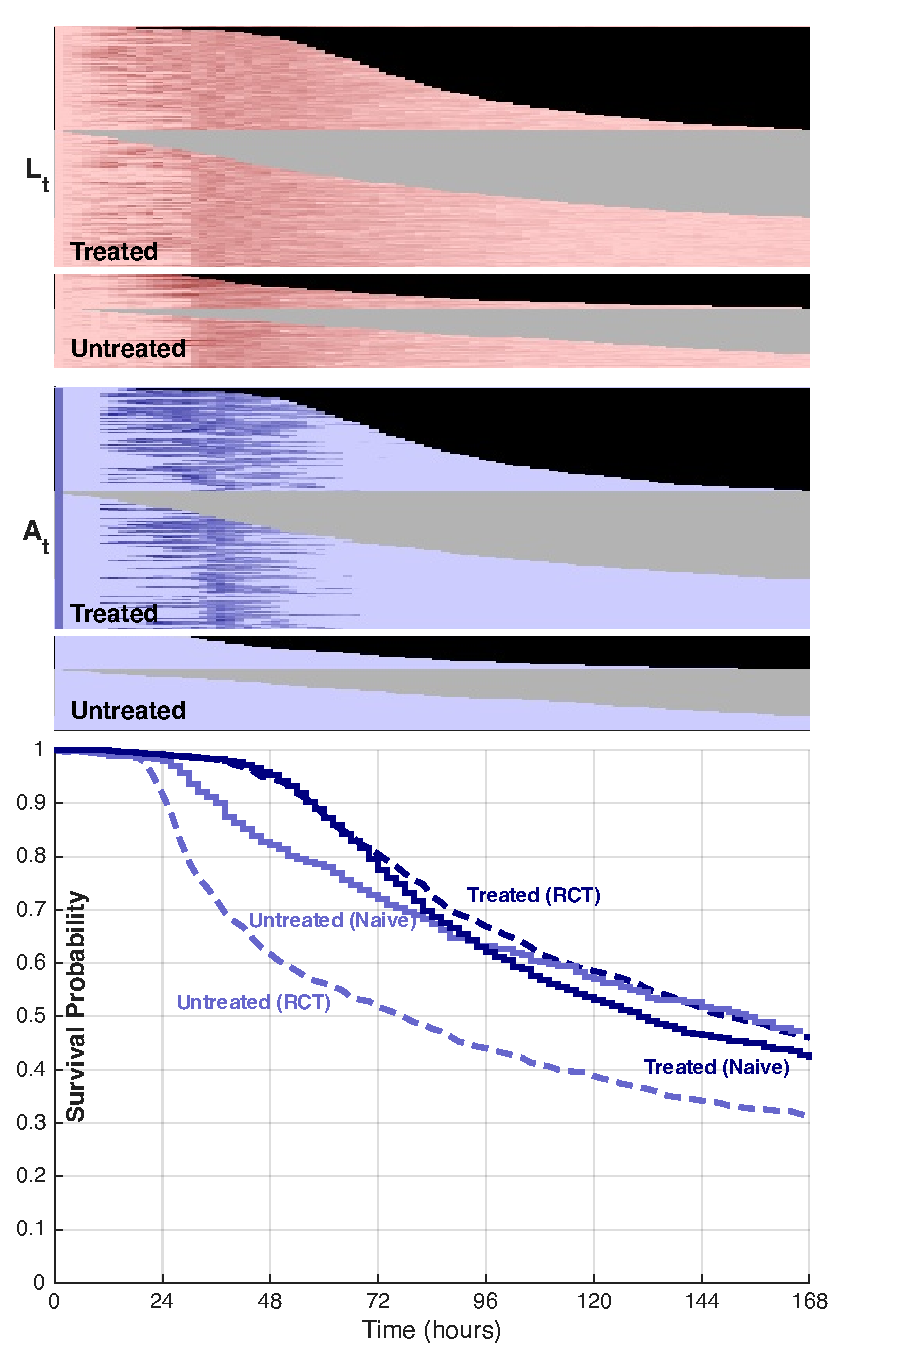
\includegraphics[width=0.68\textwidth,height=0.38\textheight,keepaspectratio, trim = 5pt 0pt 5pt 5pt, clip]{Fig4_swimmer_survival_plot_Obs_Naive.pdf}

   \caption{\textbf{Simulated trial and observational cohorts (one representative replication).}
Each row of a heatmap is one patient over 168 hours; within each block, patients are sorted by
survival time, producing the characteristic waterfall pattern. In every heatmap the treated arm is
shown in the upper block and the untreated arm in the lower block. \textbf{(A) Simulated randomized
trial} ($N = 2000$). Upper pair: epileptiform-activity burden $L_t$, light red indicating low burden
and dark red high; black indicates death. Middle pair: treatment intensity $A_t$, light blue
indicating none and dark blue high. Bottom: Kaplan--Meier survival by arm. Because assignment is
randomized and the cohort uncensored, the 168-hour survival difference is the ground-truth causal
effect of the simulation's data-generating process. \textbf{(B) Simulated observational cohort}
($N = 2000$), generated from the same disease and PK/PD models but with confounded treatment
assignment and informative censoring (gray). Baseline severity is higher among treated patients,
reflecting preferential treatment of sicker patients. Bottom: solid lines show the naive
Kaplan--Meier estimate; dashed lines reproduce the ground truth from panel~A. Values for this single
replication fall within the sampling distributions of Table~\ref{tab:multiseed}, which are what the
paper's claims rest on. All data are simulated.}
   \label{fig:swimmer_survival_rct}
\end{figure}

We emphasize that both cohorts are simulated, and that the confounding mechanism producing the
attenuation is one we specified; its magnitude is therefore a design choice rather than an empirical
finding about ICU practice. Its purpose is to provide a setting severe enough to discriminate between
estimators.

\subsection{Internal Validation: PK/PD Parameter Recovery}
\label{sec:pkpd-results}

We first evaluate the accuracy and robustness of our PKPD parameter estimation framework before assessing its performance in causal inference applications. This two-step evaluation ensures that any biases in downstream causal effect estimates can be attributed to the causal inference method rather than parameter estimation errors.

\subsubsection{Parameter Recovery Accuracy}

Figure~\ref{fig:L_prediction}A compares mean absolute percentage errors for each of the six population parameters and $k_e$ across estimation strategies. The fixed-$k_e$ oracle method (green) achieves the lowest overall MAPE (0.2\%), with zero error for $k_e$ by design, and the highest $L_0$ correlation (0.583). The two-stage corrected method (dark blue) performs nearly as well (MAPE 0.9\%, $k_e$ error 3.5\%), substantially outperforming the raw two-stage variant (MAPE 4.2\%, $k_e$ error 26.6\%) and the joint estimation approach (MAPE 22.9\%).

The superior performance of the corrected two-stage approach reflects the benefits of sequential estimation: first, establishing the natural history of the disease from untreated patients, then leveraging dose-switching variation to identify PKPD parameters. Joint estimation struggles with parameter interactions and local optima, while the raw two-stage method suffers from systematic bias in $k_e$ estimation that propagates to other parameters. The bias correction factor of 1.41, determined by regressing true $k_e$ values in the raw two-stage estimates, effectively compensates for systematic underestimation in the raw $k_e$ estimates, delivering the best practical performance for real-world applications where the true elimination constant is unknown.

\begin{figure}[htbp]
\centering
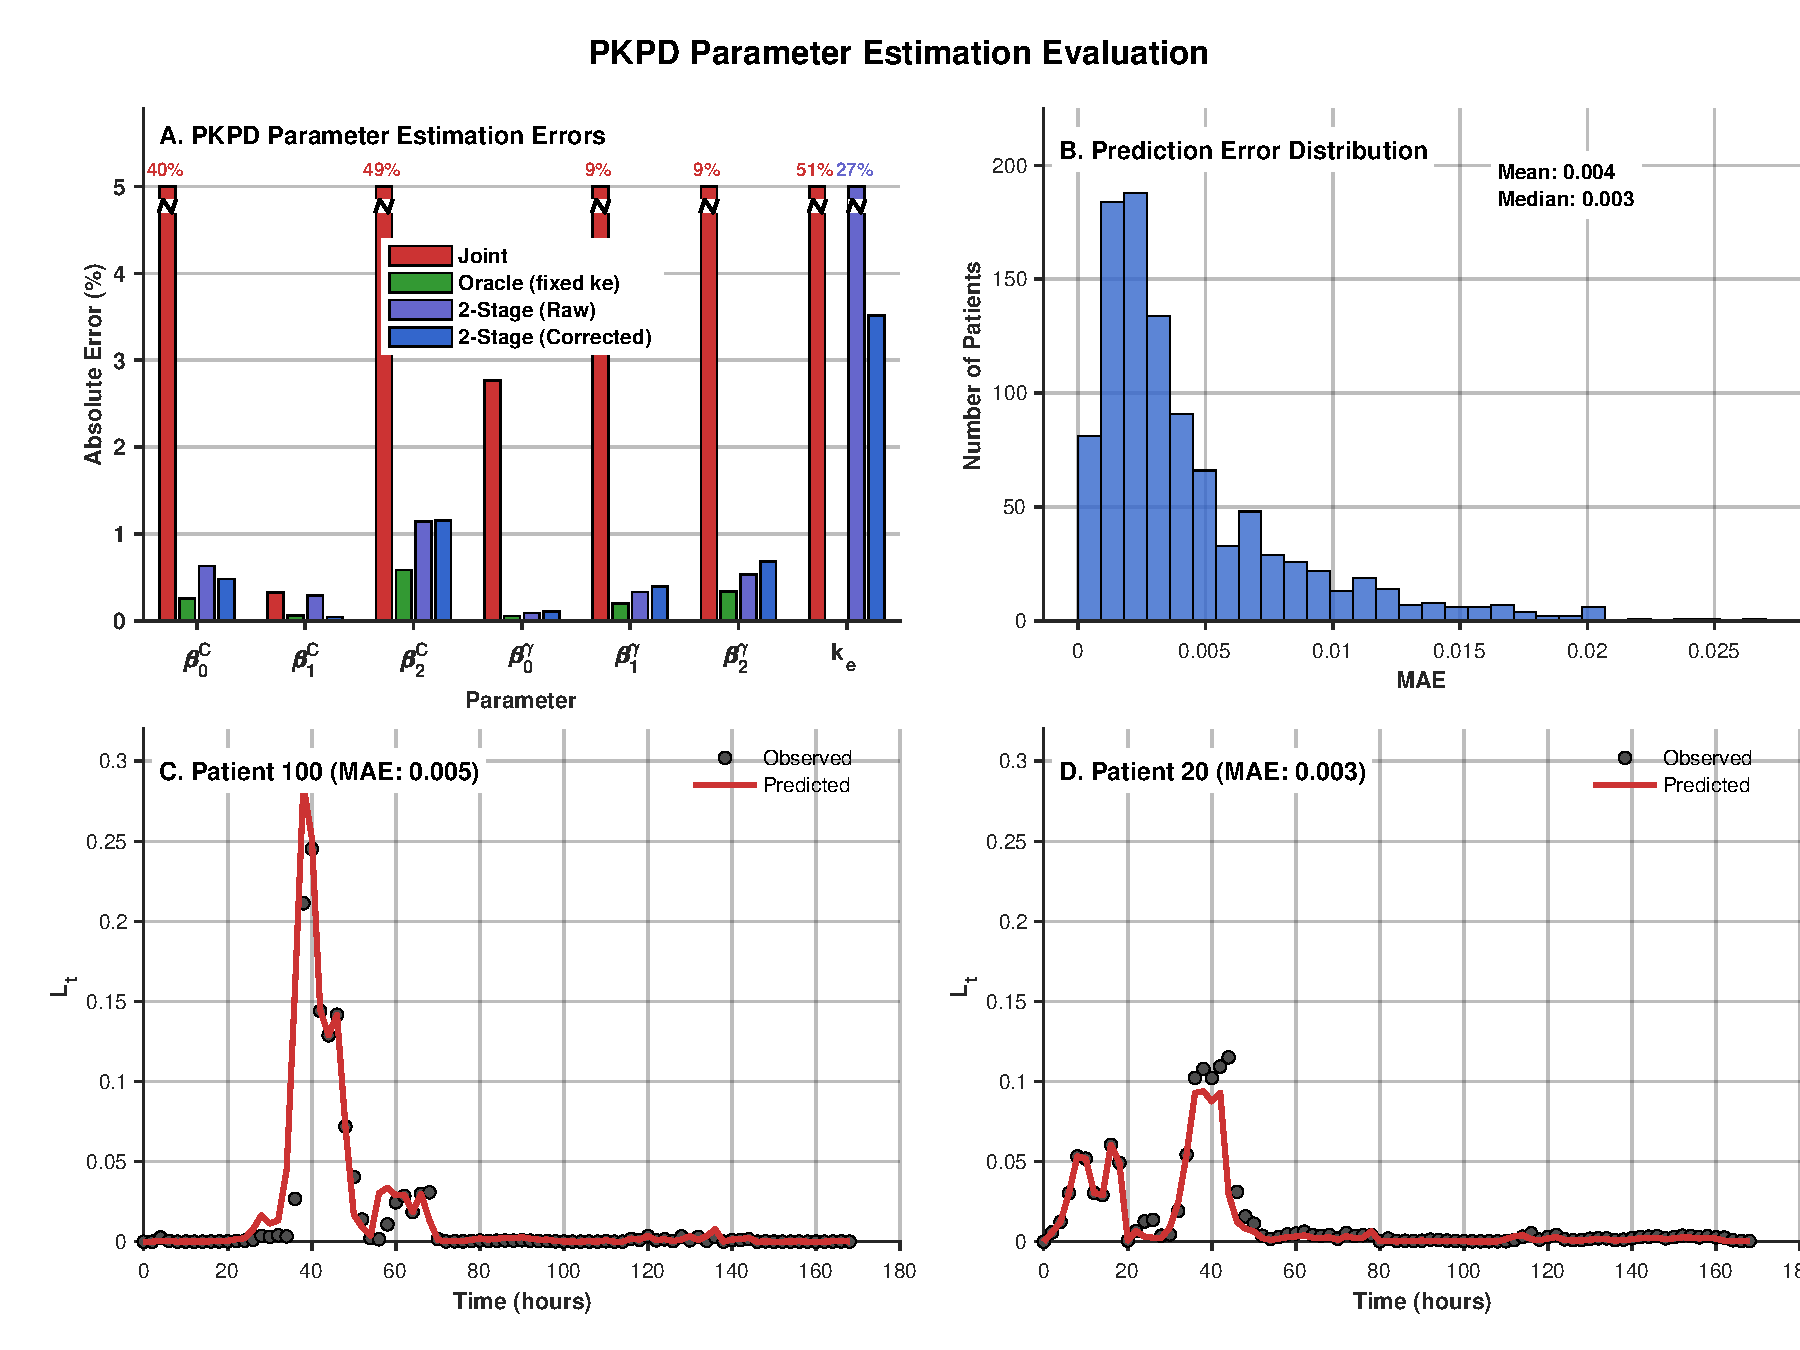
\includegraphics[width=\textwidth]{Fig_Combined_PKPD_Analysis.pdf}
\caption{(A) Absolute percentage errors in PKPD parameter estimates. Grouped bars show results for all six population parameters and $k_e$. The y-axis is truncated at 5\%; taller bars display their true values above. The oracle method (green) has zero $k_e$ error by definition. (B) Distribution of prediction accuracy values measured as mean absolute error (MAE) for $L_t$ using the PKPD parameters estimated using the 2-stage corrected method. (C,D) Two example predicted patient trajectories (red) compared with the observed values (black circles).}
\label{fig:L_prediction}
\end{figure}

\subsubsection{Predictive Performance and Model Validation}

Using the estimated PKPD parameters, we evaluated predictive accuracy for $L_t$. The corrected two-stage estimates yield visually close fits with good overall performance ($R^2 = 0.899$, Figure~\ref{fig:L_prediction}D). The prediction accuracy shows mean MAE of 0.004 (median 0.003) with mean MAPE of 52.6\% (median 45.3\%, interquartile range 37.0--56.1\%). While the MAPE values appear high, this reflects the challenge of predicting a highly suppressed signal where small absolute errors become large relative errors when $L_t$ values are near zero due to effective treatment. The strong $R^2$ value and low absolute MAE confirm that the model captures the essential dynamics despite this relative error inflation.

The mixed-effects coefficients defining how patient-specific PKPD parameters depend on covariates are recovered accurately (MAPE 0.9\%). This means we accurately recover the systematic relationships between patient characteristics (age, SOFA score) and their pharmacodynamic sensitivity. The moderate correlations between true and estimated individual patient parameters ($C_{50}$ correlation 0.532, Hill coefficient $\gamma$ correlation 0.328) reflect the inherent difficulty of recovering patient-specific random effects from limited dose-switching data, rather than errors in the underlying covariate-parameter relationships.

\subsubsection{Uncertainty Quantification}

We assessed parameter uncertainty using patient-level nonparametric bootstrap resampling ($B=1000$ replicates). Bootstrap resampling was performed at the patient level to preserve the within-patient correlation structure while allowing for realistic assessment of sampling variability. For each bootstrap replicate, we re-estimated all PKPD parameters using the corrected two-stage method.

The resulting 95\% interval for the elimination constant $k_e$ was $[0.47, 0.53]$ against a true value of $0.5$, and the intervals for the mixed-effects coefficients ($\beta^C_0$, $\beta^C_1$, $\beta^C_2$, $\beta^g_0$, $\beta^g_1$, $\beta^g_2$) were correspondingly narrow, reflecting the identification afforded by the dose-switching design.


\subsection{Internal Validation: Causal Effect Recovery}
\label{sec:gformula-results}
Having established accurate estimation of disease dynamics and PKPD parameters, we now assess whether the g-formula recovers the ground-truth causal effect of the simulation from the confounded observational cohort of Section~\ref{sec:cohorts}.

\subsubsection{Recovery of the Simulation Ground Truth}
The g-formula recovers the ground-truth effect closely despite confounding severe enough to eliminate the effect under naive analysis. For our primary comparison of aggressive treatment ($\theta = 0.1$) versus no treatment, the g-formula estimates show treated group survival of 46.3\% at 168 hours compared to 32.1\% in the untreated group, yielding an average treatment effect (ATE) of +14.2\%. 

This closely approximates the ground truth from the randomized controlled trial (treated survival 46.0\% vs. untreated 31.2\%, ATE +14.8\%), representing a recovery error of only 0.6 percentage points or 3.8\% relative error. Figure~\ref{fig:gformula_recovery} shows the estimated and ground-truth survival curves over the full follow-up. This recovery establishes that the estimator is consistent for the target parameter under the conditions of this simulation---correctly specified component models, measured confounding, and the censoring mechanism used to generate the data. It does not establish that these conditions hold in ICU data; Section~\ref{sec:misspec} discusses which of them are most likely to fail.

To assess the uncertainty quantification we repeated the entire generate--estimate--emulate procedure
across 100 independently simulated cohorts, re-estimating the mortality and natural-history models in
each. Across these replications the g-formula estimate had a standard deviation of 2.32 percentage
points, against a bootstrap standard error of 2.16 points obtained from a single cohort (ratio 0.93).
A nominal 95\% interval constructed from the bootstrap standard error contained the population
estimand in 92\% of replications (95\% CI 87--97\%), so the intervals are approximately calibrated at
the nominal level. We note that this is a lower bound on total sampling variability: as in the
bootstrap itself, the pharmacokinetic--pharmacodynamic fit is held at its point estimate rather than
re-estimated, so uncertainty in that component is not propagated into the interval.

Across the same 100 replications the estimator's mean was $+15.02$ percentage points against a mean
ground truth of $+14.30$, a bias of $+0.72$ points (95\% CI $+0.10$ to $+1.34$), or about 5\% of the
effect being estimated. The bias is small relative to the effect but statistically distinguishable
from zero, and it is upward: in this data-generating process the g-formula slightly overstates the
benefit of suppression.

One point of interpretation matters here. The g-formula estimate is obtained by forward simulation
from fitted models and therefore targets the population-level estimand rather than the realized
treatment effect of the particular cohort it was fitted on. Because a single cohort's realized effect
is itself a draw with non-trivial variability (SD 2.25 points across the replications reported here),
scoring the estimator against one cohort's realized value conflates estimator bias with that cohort's
sampling noise.

The magnitude of the correction is best read against the replicated naive estimates of Table~\ref{tab:multiseed} rather than against a single cohort. Naive Kaplan--Meier analysis retained on average only 7\% of the true effect ($+1.0$ against $+14.6$ percentage points), and in this representative cohort it indicated net harm ($-4.8\%$). The g-formula recovers the ground truth in the same data, a correction of roughly 13.6 percentage points on average and 19.6 points in the cohort shown.

\begin{figure}[H]
\centering
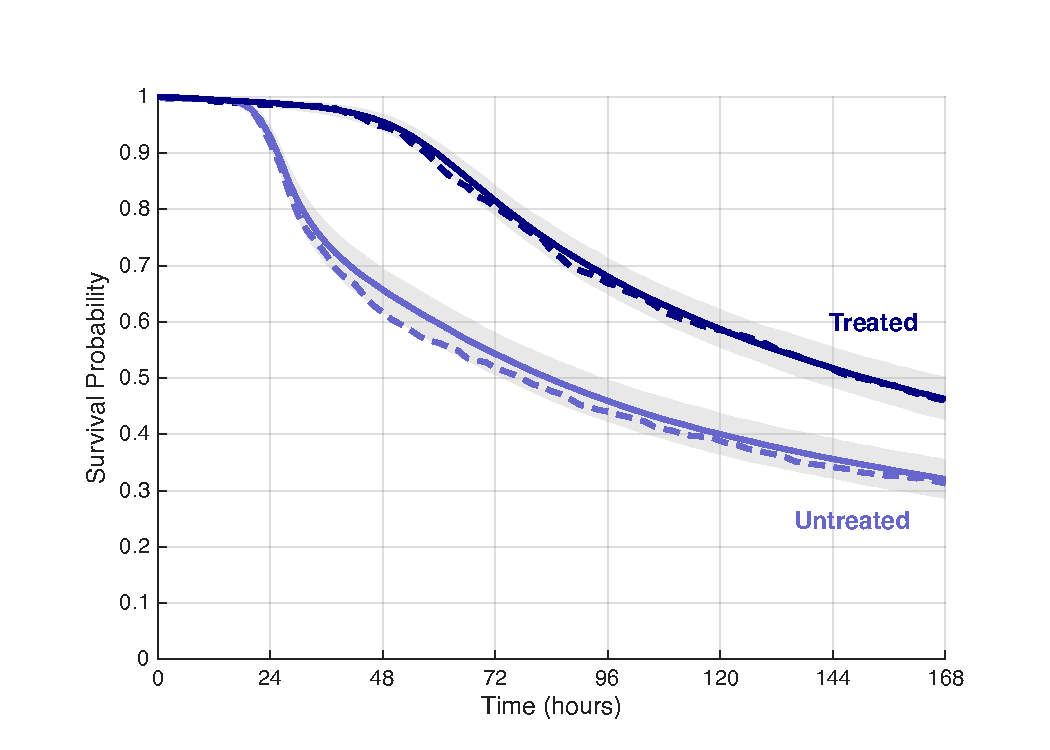
\includegraphics[width=\textwidth, trim=20pt 0pt 20pt 25pt, clip]{Fig_gformula_corrected_survival_curves.pdf}
\caption{\textbf{G-formula recovery of the simulation ground truth.} Survival probability curves over 168 hours comparing g-formula estimates from observational data (solid lines with 95\% CI) vs. ground truth from simulated RCT (dashed lines). In this representative cohort the g-formula achieves ATE $=+14.2\%$ against a ground truth of $+14.8\%$ (relative error 3.8\%). All data are simulated.}
\label{fig:gformula_recovery}
\end{figure}

\subsection{Policy-Space Exploration}
\label{sec:policy-space}

We next demonstrate the application of our framework: identifying optimal treatment strategies and revealing treatment effect heterogeneity across patient subgroups. This illustrates a second use of the framework: rather than evaluating one pre-specified contrast, it can be swept across a family of policies. In real data this would generate candidate strategies for prospective testing; here it demonstrates only that the sweep is computationally well posed and recovers the optimum of the process we specified.

\subsubsection{Optimization of Treatment Intensity}

While aggressive treatment ($\theta = 0.1$) demonstrates clear benefit over no treatment, this raises a natural question: is this particular target optimal, or could patients benefit from more or less aggressive suppression? Figure~\ref{fig:policy_space}A addresses this optimization question, revealing that our initial aggressive treatment ($\theta = 0.1$) is suboptimal.

The optimum of the simulated process occurs at $\theta = 0.02$---more aggressive suppression that yields an ATE of approximately +20.3\% at 168 hours, substantially improving upon the +14.8\% achieved with $\theta = 0.1$. Critically, the relationship between treatment intensity and survival is non-monotonic: while moderate to aggressive suppression improves outcomes, attempting to completely eliminate disease activity ($\theta = 0$) results in net toxicity with an ATE of $-8.9\%$, performing worse than no treatment.

This inverted-U relationship highlights the fundamental trade-off between disease control and treatment toxicity that characterizes many critical care interventions. The optimal treatment threshold represents the point where the marginal benefit of additional disease suppression equals the marginal harm from increased drug exposure.


\subsubsection{Patient-Specific Treatment Effects and Heterogeneity}
Figure~\ref{fig:policy_space}B compares counterfactual survival under a \emph{family of closed-loop treatment policies}, rather than across patient risk strata. In all cases, treatment follows the same closed-loop control policy, and curves differ only in the target epileptiform activity threshold $\theta$, which parameterizes the policy being evaluated.

While the simulated optimum of $\theta = 0.02$ is the best strategy for the average simulated patient, critical care populations exhibit substantial heterogeneity in disease and treatment susceptibility. Figure~\ref{fig:policy_space}B systematically explores how optimal treatment strategies vary across patient types, indexed by their susceptibility to cumulative disease harm (horizontal axis) and cumulative drug harm (vertical axis).

Across the simulated grid of disease-harm and drug-harm susceptibilities, the policy contrast ranges from $-8.9\%$ to $+71.6\%$. The boundary separating regions where suppression helps from regions where it harms is a direct consequence of the two-parameter harm model specified in Section~\ref{sec:outcome-model}; its position carries no information about where such a boundary would lie in patients. What the figure demonstrates is that the framework \emph{localizes} such a boundary when one exists, which is the property that would be useful in real data.

Applying the threshold that is optimal for each simulated patient, rather than a single population-wide threshold, yields a policy contrast of $+31.7\%$ versus $+20.3\%$. That an individualized policy outperforms a uniform one inside a simulation with heterogeneous, known patient parameters is expected by construction rather than surprising: the individualized policy has access to the generating parameters. The quantity of interest is not the margin itself but whether the framework recovers the individualized optimum when those parameters must be estimated, which is what Section~\ref{sec:pkpd-results} assesses.

\begin{figure}[p]
\centering
\noindent\textbf{(A) Sweep over the target threshold $\theta$}\par\vspace{0.2em}
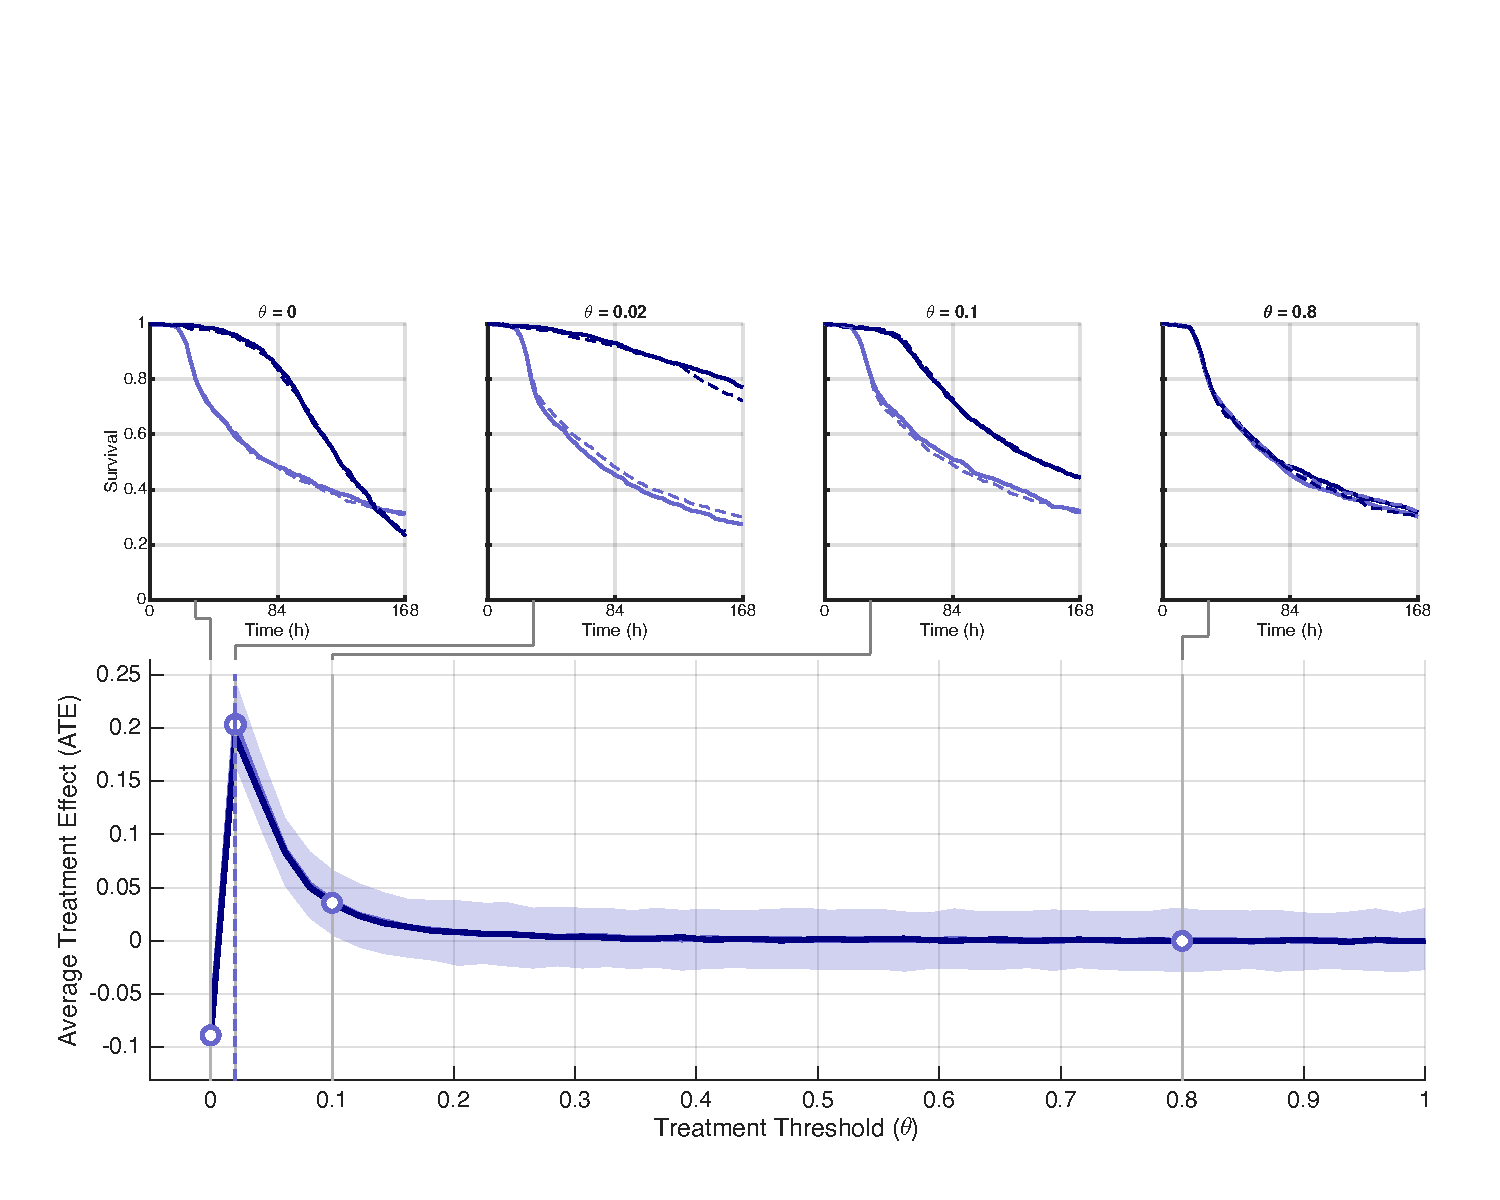
\includegraphics[width=\textwidth,height=0.40\textheight,keepaspectratio]{Fig_optimization_curves_with_survival.pdf}

\vspace{1.2em}

\noindent\textbf{(B) Policy contrast by simulated patient type}\par\vspace{0.2em}
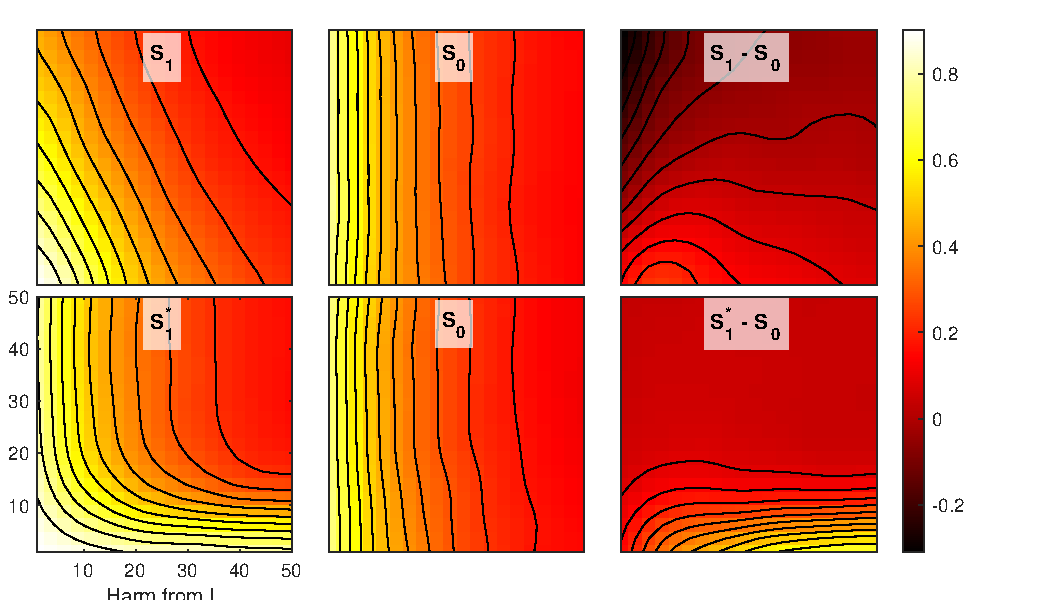
\includegraphics[width=\textwidth,height=0.40\textheight,keepaspectratio, trim=0pt 5pt 0pt 0pt, clip]{Fig_heatmap_figure.pdf}
\caption{\textbf{Exploring the space of closed-loop policies.} \textbf{(A)} Sweep over the family of
policies indexed by the target threshold $\theta$. Top: counterfactual survival curves under
different $\theta$. Bottom: policy contrast as a function of $\theta$, with the optimum of the
simulated process at $\theta = 0.02$ (contrast $+20.3\%$) and net toxicity under complete suppression
($\theta = 0$). The inverted-U shape reflects the benefit--toxicity trade-off specified in the
outcome model. \textbf{(B)} Policy contrast as a function of simulated patient type, indexed by
susceptibility to cumulative disease harm ($x$-axis) and cumulative drug harm ($y$-axis). Top row:
survival under treatment target $\theta = 0.1$ ($S_1$), under no treatment ($S_0$), and their
difference. Bottom row: survival under individualized optimal thresholds ($S_1^*$) and the
corresponding contrast $S_1^*-S_0$. The boundary separating benefit from harm is a direct consequence
of the two-parameter harm model and carries no information about where such a boundary would lie in
patients. All data are simulated.}
\label{fig:policy_space}
\end{figure}













































\subsection{Robustness Analyses}
\label{sec:robustness}

\paragraph{Robustness to unmeasured confounding.}
Across the \(5 \times 5\) (\(\delta_A\), \(\delta_Y\)) grid, with three seeds per cell at
\(N = 1500\) patients, the g-formula ATE retained the correct sign in every cell; no
sign flip was observed. The largest mean bias across cells was approximately
\(+10\) percentage points, at \((\delta_A = 0.5, \delta_Y = 0)\). The baseline (honest)
cell \((\delta_A = 0, \delta_Y = 0)\) showed a mean bias of about \(+4.6\) pp, which is
within the expected finite-sample seed variance at this \(N\) and illustrates the
intrinsic variability of the estimator rather than a systematic effect of \(U\).
Importantly, there is no monotonic pattern in which larger \(U\) effects produce larger
bias, suggesting that within the tested range the g-formula's estimate is primarily
noise-limited rather than bias-limited. The Ding--VanderWeele E-value for the honest ATE
was \(1.46\), meaning an unmeasured confounder would need a risk ratio of at least 1.46
with both treatment assignment and mortality to fully account for the observed effect.
Full results appear in \texttt{sensitivity/nuc\_injection/nuc\_results.mat}.

\paragraph{Robustness to EEG measurement error.}
Small amounts of measurement error on \(L_t\) had modest effect on the recovered ATE: at
\(\sigma = 0.025\) the bias remained within stochastic seed variability. Above
\(\sigma = 0.05\) the two-stage PKPD estimator fit-failed on a substantial fraction of
cohorts because the signal-to-noise ratio in \(L_t\) became too low for stable
identification of \(C_{50}\) and \(\gamma\). This sets a practical requirement that the
EEG-severity proxy used in the planned real-data analysis be measured with noise well
below this threshold.

\paragraph{Robustness to censoring mechanism.}
Under the baseline censoring regime used in the paper, the g-formula bias was
\(-0.6~\mathrm{pp}\) relative to the RCT truth. Under MCAR censoring at a low rate, bias
was approximately \(+8~\mathrm{pp}\); under strongly outcome-dependent censoring (5\% of
person-time censored in a manner correlated with both disease severity and treatment
intensity), bias grew to \(+17~\mathrm{pp}\). This sensitivity is expected: when
censoring is strongly informative and the observed data do not capture what drives
loss-to-follow-up, the g-formula's assumption of conditional independent censoring is
violated, and bias increases. For the planned real-data analysis, rigorous
characterization of the censoring mechanism (protocol deviations, withdrawal of care,
transfer out) will be essential.

\subsection{Methodological Benchmarking against IPTW, MSM, and Naive KM}
\label{sec:benchmark}
Table~\ref{tab:benchmark} reports the 168-hour ATE estimates from four methods on the same
simulated observational cohort (\(N = 2000\)), with 95\% bootstrap CIs.

\begin{table}[H]
\centering
\begin{tabular}{lrrr}
\toprule
Method                  & ATE at 168h & 95\% CI         & Bias vs truth \\
\midrule
RCT truth               & $+14.8\%$   & ---             & ---           \\
Naive Kaplan--Meier     & $-4.8\%$    & $[-11.4, -0.2]$ & $-19.6$~pp    \\
Stabilized IPTW         & $+16.6\%$   & $[+2.5, +27.4]$ & $+1.9$~pp     \\
MSM (baseline-weighted) & $+31.6\%$   & $[+17.2, +41.7]$& $+16.8$~pp    \\
\textbf{CICADAS g-formula} & $\mathbf{+14.5\%}$ & $[\mathbf{+7.4, +20.8}]$ & $\mathbf{-0.3~pp}$ \\
\bottomrule
\end{tabular}
\caption{Four-method comparison of 168-hour ATE recovery from the same simulated observational cohort. Bootstrap 95\% CIs: 200 replicates for naive KM/IPTW/MSM; 1000 replicates for the CICADAS g-formula. The CICADAS g-formula is the only estimator whose point estimate lies within one standard error of the RCT ground truth. All four estimators are computed on one shared cohort so that the comparison is like-for-like; the g-formula value here ($+14.5\%$) therefore differs slightly from the $+14.2\%$ reported in Section~\ref{sec:gformula-results}, which is computed on an independently simulated cohort. The 0.3-point difference is Monte Carlo variation between cohorts (Table~\ref{tab:multiseed}). All data are simulated.}
\label{tab:benchmark}
\end{table}

The CICADAS g-formula is the only estimator among the four whose point estimate is within
one standard-error of the RCT truth. IPTW is approximately correct but the propensity
model produced extreme weights (maximum 131; 99th percentile 2.74) reflecting
near-positivity violation for the continuous state-dependent dosing in this simulation.
This is empirical evidence for the conceptual argument made in Section~\ref{sec:positivity} that IPTW is
ill-suited to continuous-treatment dynamic policies over long horizons.

This comparison is methodological benchmarking, not evidence of clinical superiority. The g-formula
implementation here is correctly specified with respect to the process that generated the data, while
the IPTW and MSM implementations are standard off-the-shelf specifications; a comparison in which one
estimator knows the true functional form and its competitors do not is informative about
implementation, not about which method to prefer in real data. The IPTW result is nonetheless
instructive on its own terms: the propensity model produced extreme weights (maximum 131) reflecting
near-violation of positivity for continuous state-dependent dosing, and that difficulty is intrinsic
to the setting rather than to our implementation. In real data, where no method is correctly
specified, the ordering could differ. The MSM with
baseline-only stabilized weights is substantially biased, overestimating the ATE by
approximately 17 percentage points; a time-varying MSM that also reweights for time-
varying confounders would in principle do better, but would itself suffer from the same
near-positivity issue with extreme weights.

\section{Discussion}
\label{sec:discussion}

\subsection{What This Study Shows, and What It Does Not}

CICADAS is an end-to-end modeling, estimation, and simulation framework for emulating randomized
trials of dynamic treatment policies from longitudinal observational data. In this paper we
specified the framework, implemented it in MATLAB and Python, and evaluated it entirely by internal,
simulation-based validation.

Within that evaluation, three things were shown. First, in synthetic ICU cohorts with confounding by
indication severe enough to eliminate---and in a substantial fraction of replications reverse---the
apparent treatment benefit, the parametric g-formula recovers the ground-truth policy contrast
closely, while naive Kaplan--Meier, stabilized IPTW, and a baseline-weighted marginal structural
model do not. Second, the sequential estimation procedure---natural history from untreated patients,
PK/PD parameters from dose-switching patients, mortality from the full cohort---recovers the
generating parameters accurately, and the corrected two-stage estimator approaches oracle
performance. Third, the estimator's behavior degrades in characterizable ways under injected
unmeasured confounding, EEG measurement error, and misspecified censoring.

None of this constitutes evidence about anti-seizure treatment in patients. Every number reported
here is a property of a data-generating process that we specified, recovered by an estimator that we
also specified; the two share structural assumptions, as Section~\ref{sec:misspec} discusses. The
appropriate reading is that the framework is \emph{methodologically feasible}---the estimation
problem is solvable, the computations are tractable at realistic cohort sizes, and the failure modes
are identifiable---and that its clinical utility is entirely undetermined.

\subsection{Methodological Contributions}

CICADAS addresses three challenges in ICU causal inference through integrated solutions: mechanistic
modeling captures underlying disease biology and drug effects, sequential parameter estimation
leverages natural treatment variation in clinical practice, and the parametric g-formula simulates
counterfactual outcomes under alternative policies. The corrected two-stage estimation approach
achieves near-oracle accuracy for key PK/PD parameters, while the g-formula removes the substantial
bias present in standard survival analyses of the same simulated data.

Causal effect recovery depends on accurate PK/PD parameter estimation, since these parameters
determine the mapping from treatment decisions to disease suppression and downstream mortality. In
these simulations, sufficient dosing variation was necessary for stable identification, whereas data
from constant closed-loop control provided insufficient dynamic range for reliable
estimation---motivating our use of dose-switching patients for parameter estimation. This is a
design insight that transfers directly to any real-data application of this class of method.

\subsection{Model Misspecification and the Shared-Structure Problem}
\label{sec:misspec}

The most important limitation of a simulation study of this design is that the data-generating
process and the estimation models are not independent. Both use a one-compartment pharmacokinetic
approximation; both represent pharmacodynamic effect as multiplicative suppression of disease burden
through a Hill function; both express mortality as a discrete-time hazard depending on cumulative
disease and cumulative drug burden through the same functional form; and both draw natural history
from the same parametric family. When the estimator is handed data generated under exactly the
structure it assumes, recovering the truth demonstrates that the estimator is consistent and that
the numerical implementation is correct. It does not demonstrate that the estimator is robust,
because nothing was misspecified.

We therefore regard the recovery results as characterizing an \emph{upper bound} on achievable
performance rather than an expected performance in practice. The sensitivity analyses in
Section~\ref{sec:robustness} relax this in three specific directions---an unmeasured confounder
entering both treatment assignment and mortality, additive measurement error on the EEG severity
proxy, and alternative censoring mechanisms---and the framework's behavior under each is
informative. But three named departures are not robustness to misspecification in general. In
particular, we did not test: the wrong number of PK compartments; non-monotone or saturating
dose--response departing from the Hill form; time-varying PK/PD parameters (which occur clinically
with changing renal and hepatic function, and with autoinduction); drug--drug interaction in
patients receiving multiple agents; or a mortality hazard depending on the \emph{pattern} of
exposure rather than its cumulative total. Any of these is plausible in real ICU data, and each
would bias the estimator in a direction that our current experiments cannot predict.

A distinct concern is transportability. Even a correctly specified model, fit in one cohort,
estimates a quantity specific to that cohort's case mix, drug formulary, monitoring intensity, and
---critically in critical care---its local practice around withdrawal of life-sustaining therapy.
Between-center variation in these is substantial, and it enters the estimand rather than merely the
variance. Estimates from a single center should not be assumed to transport, and a multicenter
analysis should report between-center heterogeneity rather than pooling over it.

\subsection{Conditions Required to Apply CICADAS to Real Data}
\label{sec:conditions}

The framework is not applicable to an arbitrary longitudinal ICU dataset. Six conditions must hold,
and each is checkable before any causal estimate is produced. We state them explicitly because a
framework whose preconditions are left implicit invites misapplication.

\begin{enumerate}\setlength{\itemsep}{3pt}
\item \textbf{Treatment overlap over the policy range of interest.} Every policy compared must have
support: for each patient stratum and each time point, the observed data must contain patients
receiving treatment intensities consistent with the policy being evaluated. In practice this means
examining the empirical distribution of dose conditional on severity and confirming it is
non-degenerate over the range of $\theta$ being swept. Where it is not, the corresponding portion of
the policy curve is extrapolation from the parametric model and should be reported as such rather
than plotted alongside supported regions (see Section~\ref{sec:structural-limits}).

\item \textbf{Measured confounding sufficient for sequential exchangeability.} The covariates
recorded must capture what actually drives dose escalation---not only severity and vital signs, but
sedation goals, neurologic examination findings, and goals-of-care status. The last of these is
routinely absent from structured data and is plausibly a strong confounder, since a decision to
limit escalation and a high mortality risk share a common cause. Negative-control
outcomes~\cite{lipsitch2010negative} and multiple propensity specifications should accompany any
real-data estimate.

\item \textbf{Dosing variation adequate to identify PK/PD parameters.} Section~\ref{sec:pkpd-results}
shows that patients under stable closed-loop control carry little information about drug effect:
identification requires within-patient variation in exposure. A cohort in which dosing is uniformly
protocolized is, for this purpose, uninformative---the framework requires the very practice
variation that motivates it. We recommend reporting the proportion of person-time spent with
$x_t/C_{50}$ in a range that supports identification, as a design diagnostic prior to estimation.

\item \textbf{A severity readout of adequate fidelity.} Our measurement-error experiments indicate
that the two-stage PK/PD estimator fails to converge on a substantial fraction of cohorts once noise
on the severity signal exceeds $\sigma \approx 0.05$. This is a concrete, quantitative precondition
on the EEG quantification pipeline, and it should be verified against that pipeline's known error
characteristics before analysis. Section~\ref{sec:eeg-readout} addresses the harder question of
whether a scalar readout is the right object at all.

\item \textbf{A characterized censoring mechanism.} Our censoring experiments show bias growing to
approximately $+17$ percentage points under strongly outcome-dependent censoring. In ICU data, loss
to follow-up is generated by transfer, monitoring discontinuation, and withdrawal of care---the last
of which is not plausibly independent of prognosis. The mechanism must be characterized and modeled,
not assumed.

\item \textbf{Subgroups represented in sufficient number.} Policy comparisons within a stratum
require that the stratum contain enough patients, with enough treatment variation, to fit the
component models. Strata failing this should be reported as indeterminate rather than as showing no
effect.
\end{enumerate}

\subsection{What the Framework Structurally Cannot Do}
\label{sec:structural-limits}

Two limits are structural rather than statistical, and no amount of data or computation removes
them.

The first bounds the credible policy space. CICADAS produces empirically defensible estimates only
for policies with support in the observed data; policies outside that range are extrapolations from
the fitted parametric models, and their apparent precision is an artifact of the parametric form
rather than evidence. This has a direct consequence for the threshold optimization presented in
Section~\ref{sec:policy-space}. Sweeping $\theta$ toward zero corresponds to a degree of suppression
that may simply not occur in routine practice, and in real data the corresponding portion of the
curve would be model-based conjecture. The honest output of a real-data application is therefore two
maps rather than one: a map of estimated treatment-effect heterogeneity, and a map of where the data
can speak at all. Regions where the observational data are structurally silent should be flagged for
prospective study, never presented as null findings.

The second limit is more fundamental and deserves to be stated plainly. Because the framework learns
the effects of treatment from variation in treatment that has already occurred, it can only ever
interrogate the space of therapies, mechanisms, and timing strategies embodied in current practice.
It can find the best policy within that space; it cannot find a policy outside it. A genuinely novel
agent, a mechanism no current drug targets, or a timing strategy nobody has attempted---the
disruptive interventions that produce real advances in clinical care---are invisible to it by
construction. This is not a deficiency to be engineered away; it is the definitional boundary
between learning from observation and learning from experiment. Randomized trials remain the only
instrument capable of evaluating interventions that have never been tried, and the appropriate
relationship between CICADAS and trials is therefore complementary: the framework is a tool for
allocating trial resources efficiently within known therapeutic space, not a substitute for the
trials that extend it.

\subsection{The EEG-Derived Treatment Target}
\label{sec:eeg-readout}

The framework assumes the availability of a scalar severity readout $L_t$ that can be tracked
continuously and titrated against a threshold. This assumption is doing more work than it appears
to, and we regard it as the most substantial obstacle to real-world deployment.

Clinically distinct electrographic states are not interchangeable instances of a single quantity.
Several brief focal seizures and one prolonged ictal episode may integrate to the same burden while
carrying different prognostic implications; focal and generalized activity differ in mechanism and
in likely response to systemic suppression; and identical ictal burden on a continuous, reactive
background versus a burst-suppressed or attenuated background reflects different underlying brain
states and, plausibly, different treatment benefit. There is also an irreducible measurement problem
beneath the modeling one. Expert electroencephalographers identifying seizures and rhythmic and
periodic patterns---precisely the categories a severity readout would have to be built
from---agree only moderately with one another~\cite{jing2023interrater}. A scalar target inherits
that irreducible label noise before any modeling assumption is made. Collapsing all of this to one
number then imposes a further substantive and currently unvalidated assumption: that harm is a
monotone function of a scalar summary, and that the summary is sufficient for the treatment
decision.

There is a practical problem alongside the conceptual one. Retrospective ICU datasets frequently
lack granular quantitative EEG; the recorded product is often a narrative report at daily resolution
rather than a time series at the resolution titration requires. Where raw EEG is available, deriving
a continuous target requires an automated quantification pipeline whose error characteristics are
known and whose output has been validated against outcomes---and, per
Section~\ref{sec:conditions}, whose noise falls below the threshold at which our estimation
procedure destabilizes.

The consequence is that optimizing $\theta$ is mathematically well posed inside the simulation while
being potentially uninterpretable outside it. A real deployment must therefore either commit to a
specific, prospectively validated scalar readout and defend that choice on its own evidence, or
generalize the framework so that severity is a vector or a pattern type rather than a scalar. The
latter is a substantial extension: it changes the controller, the identification argument, and the
policy space simultaneously. We regard resolving this as a prerequisite for, rather than a
refinement of, clinical application.

\subsection{Clinical Heterogeneity and the Mismatch with the Simulation}

The present simulation treats all critically ill patients with electrographic seizures as a single
population. In reality, causes of ICU seizures and the underlying pathophysiology are heterogeneous,
and the likelihood that anti-seizure treatment changes outcomes plausibly differs across etiologies.
Clinically important categories include: (i) post-anoxic encephalopathy, where widespread ischemic
injury from cardiac arrest may render treatment ineffective regardless of seizure
burden~\cite{rossetti2005refractory,ruijter2022treating}; (ii) primary structural injury
(large-artery ischemic stroke, intracerebral hemorrhage, traumatic brain injury, brain tumor), where
seizures arise from focal cortical damage and the benefit of aggressive suppression may depend on
lesion type and location~\cite{claassen2004detection,vespa2005continuous}; (iii) systemic,
metabolic, and septic encephalopathy, where seizures are often transient and reverse with treatment
of the underlying condition, so that aggressive anti-seizure therapy may add toxicity without
benefit~\cite{sutter2016status}; and (iv) primary epileptic populations with non-convulsive status
epilepticus, where conventional anti-seizure protocols are more likely to be
effective~\cite{trinka2015definition,husain2018randomized}. The causal structure---which covariates
confound, which mediate, and which modify treatment effects---likely differs across these groups.

We note explicitly that these etiologic distinctions are \textbf{not represented in the present
simulation}. The heterogeneity in our data-generating process is parametric---patients differ in
susceptibility to cumulative disease harm and to cumulative drug harm---rather than mechanistic.
Parametric heterogeneity of this kind is sufficient to exercise the machinery of stratified policy
estimation, but it is not the same thing as the clinical heterogeneity we invoke to motivate the
framework's relevance, and it should not be read as evidence that the framework handles that
heterogeneity. A simulation that did so would need distinct disease-dynamics and benefit--harm
structures per etiology, including etiologies in which treatment is futile at any dose, and would
need to test whether the estimator recovers effects separately within strata of markedly unequal
size. We regard building that simulation as a necessary step before real-data deployment, and it is
not attempted here.

Similarly, on the harm side of the trade-off, the present simulation represents treatment harm only
as a concentration-dependent contribution to the mortality hazard. A complete representation in a
real clinical deployment would separate concrete harms that clinicians weigh in practice:
sedation-related hypotension and the need for vasopressor support, prolonged mechanical ventilation
and the associated risk of ventilator-associated pneumonia, delayed weaning and ICU length of stay,
delayed neuroprognostication in post-arrest patients, and drug-specific toxicities (e.g., propofol
infusion syndrome~\cite{kam2007propofol}, thrombocytopenia with valproate, hepatic failure with other
agents~\cite{perucca2012adverse}). The framework's outcome model can be extended to treat each of
these as a distinct competing or intermediate outcome, and we regard this as a priority in the
real-data application.

\subsection{Limitations}

Beyond the structural issues above, our simulations assume simplified patient heterogeneity and
one-compartment pharmacokinetics, whereas real applications may require additional covariates and
more complex models. The identification argument assumes no unmeasured confounding of the
treatment--outcome relationship at each time point; Section~\ref{sec:robustness} quantifies the
bias induced by violations of a specific parametric form, but cannot establish that the assumption
holds in any real dataset. Finally, our benchmarking comparisons are subject to the caveat stated in
Section~\ref{sec:benchmark}: our g-formula implementation is correctly specified with respect to the
generating process while its competitors are off-the-shelf specifications, so the ordering we
observe should not be read as a general ranking of methods.

\subsection{External Validation}
\label{sec:external-validation}

The necessary next step is external validation in real ICU EEG data, and we describe it here
strictly as future work that does not support any claim in the present manuscript. We are assembling
a multicenter cohort of ICU patients undergoing continuous EEG monitoring for this purpose. That
analysis will be the first test of whether the preconditions in Section~\ref{sec:conditions} are
satisfiable in practice---whether overlap is adequate, whether the measured covariates suffice,
whether dosing variation identifies PK/PD parameters, and whether a severity readout of the required
fidelity can be constructed. It is entirely possible that they are not, and a negative answer on any
of them would be an informative result about the limits of this class of method.

Only if those preconditions are met does the question of clinical utility arise, and even then the
framework's output would be a set of hypotheses about which patients and which treatment intensities
merit prospective evaluation---not treatment recommendations. Establishing clinical utility would
require a subsequent trial testing a CICADAS-derived strategy against usual care. Until such a trial
is conducted, the framework's value is methodological.

\section{Conclusion}
\label{sec:conclusion}

We have presented CICADAS, a computational framework that couples the parametric g-formula with
mechanistic PK/PD modeling, disease dynamics, and closed-loop treatment policies to emulate
randomized trials of dynamic anti-seizure strategies from longitudinal observational data. Evaluated
on synthetic ICU cohorts with known ground truth, the framework recovers the generating causal
effect under confounding severe enough to eliminate the apparent treatment benefit, outperforms
standard IPTW and marginal structural model implementations on the same simulated data, and degrades
in characterizable ways under unmeasured confounding, measurement error, and informative censoring.
We have specified the conditions a real dataset must satisfy for the framework to apply---treatment
overlap across the policy range, sufficient measured confounding, dosing variation adequate to
identify PK/PD parameters, a severity readout of adequate fidelity, a characterized censoring
mechanism, and adequately represented subgroups---and we have set out what the framework
structurally cannot do, including evaluating therapies outside current practice.

These results establish methodological feasibility and provide a benchmarked implementation. They do
not establish clinical utility. Because our simulated data and our estimation models share
structural assumptions, and because no real patient data were analyzed, whether CICADAS produces
valid causal estimates in ICU practice remains an open question that only independent external
validation, followed by prospective evaluation of any resulting hypothesis, can answer.

% Revision-added metadata sections: CRediT, Funding, COI, Ethics, AI disclosure.
% Data and Code Availability has been moved to the STAR Methods
% Resource Availability subsection (resource_availability.tex).

\section*{Author Contributions}

Following the CRediT taxonomy:

\noindent\textbf{Conceptualization:} A.F.S., J.A.K., M.B.W., S.F.Z.\\
\textbf{Methodology --- causal inference:} H.P., A.V., C.R., D.C., M.B.W.\\
\textbf{Methodology --- mechanistic pharmacokinetic--pharmacodynamic modeling:} M.M., Z.A., P.C., S.F.Z., M.B.W.\\
\textbf{Software --- simulation engine and estimation code:} M.M., T.W., P.W., H.S., N.T., M.B.W.\\
\textbf{Validation --- verification of simulation outputs and estimator recovery:} M.M., P.W., T.W., H.S., N.T.\\
\textbf{Formal analysis:} M.M., T.W., P.W., S.S., Z.A., M.B.W.\\
\textbf{Clinical framing:} A.F.S., J.A.K., S.F.Z., M.B.W.\\
\textbf{Writing --- original draft:} M.M., T.W., P.W., S.S., M.B.W.\\
\textbf{Writing --- review and editing:} All authors.\\
\textbf{Visualization:} M.M., P.W., T.W., M.B.W.\\
\textbf{Supervision:} S.F.Z., A.F.S, J.A.K., M.B.F., M.B.W.\\
\textbf{Project administration:} S.F.Z., M.B.W.\\
\textbf{Funding acquisition:} S.F.Z., J.A.K., A.F.S., M.B.W.

\noindent All authors reviewed and approved the final version of the manuscript. This study used
simulated data only; no data were collected from human or animal subjects, and the CRediT roles of
Investigation and Data curation therefore do not apply.

\section*{Funding}

This work was supported by grants from the U.S. National Institutes of Health:
RF1AG064312, RF1NS120947, R01AG073410, R01HL161253, R01NS126282, R01AG073598,
R01NS130119, and R01NS131347.

\section*{Declaration of Competing Interests}

M.\ Brandon Westover is a co-founder of, scientific advisor and consultant to, and
holds personal equity in Beacon Biosignals. The remaining authors declare no
competing interests.

\section*{Ethics}

All analyses reported in this paper use simulated data only; no human-subjects data
were used. The in-progress application of this framework to ICU EEG data at
Massachusetts General Hospital, Brigham and Women's Hospital, and Beth Israel Deaconess
Medical Center is conducted under protocols approved by the Beth Israel Deaconess
Medical Center IRB (\#2022P000481, \#2022P000417) and the Mass General Brigham IRB
(\#2013P001024), with waivers of informed consent for retrospective data analysis.
No prospective data acquisition or participant recruitment was performed.

\section*{Declaration of Generative-AI Use}

No generative-AI tools were used in the preparation of this manuscript.


\section*{Data and Code Availability}
All data analyzed in this paper are simulated; no human-subjects data were used. The complete
simulation, estimation, and analysis code is openly available in both MATLAB and Python at
\url{https://github.com/bdsp-core/cicadas} under the MIT license, together with the scripts that
regenerate every figure and table in this paper and in the Supplementary Material. The version
accompanying this paper is archived as release \texttt{v1.0.0}
(\url{https://github.com/bdsp-core/cicadas/releases/tag/v1.0.0}); readers seeking to reproduce the
results reported here should use that tag rather than the development branch. The multi-seed
replication reported in Section~\ref{sec:cohorts} is reproduced by the drivers in the
\texttt{multiseed/} directory of that repository. The two implementations use different random number
generators (Mersenne Twister and PCG64) and therefore produce different individual cohorts from the
same nominal seed; Section~\ref{sec:cohorts} reports the agreement between them across replications.

% Bibliography
\bibliographystyle{plain}
\bibliography{references}

\end{document}
